\begin{frame}[plain]{GPU-based systems}
  
  % \begin{itemize}
  % \item[\dg{$\blacktriangle$}] 5x more floating-point performance than CPUs
    %% \item[\db{$\blacktriangle$}] Energy efficient

  \vspace{-0.8cm}

  % \item[\dr{$\blacktriangledown$}] Efficient on computationally
    % intensive kernels.
  % \item[\dr{$\blacktriangledown$}] Requires large granularity tasks to
    % feed GPUs resources.
  % \item[\dr{$\blacktriangledown$}] Memory transfers generally costly.
  % \end{itemize}  
  
  \begin{columns}
    \begin{column}{0.72\textwidth}
      \begin{itemize}
      \item Very high computing power ($O(1)$ Tflop/s)
      \item Very high memory bandwidth ($O(100)$ GB/s)
      \item Very convenient Gflops/s/Watt ratio ($O(10)$)  
      \end{itemize}
    \end{column}
    \begin{column}{0.28\textwidth}
      \begin{center}
        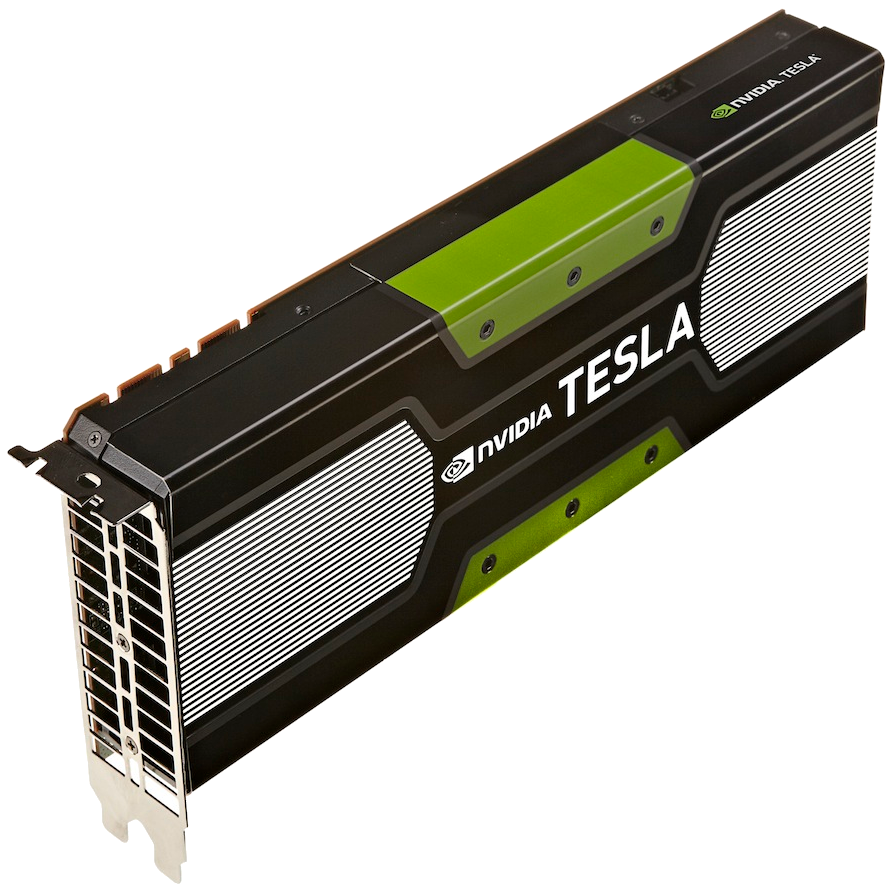
\includegraphics[width=0.9\textwidth]{figures/tesla.png}
      \end{center}
    \end{column}
  \end{columns}
  

  \begin{block}{Objective}
    Exploit \dr{heterogeneity} (i.e. take advantage of the diversity of
    resources) to accelerate the multifrontal QR factorization.
  \end{block}

  \vspace{0.2cm}

  \uncover<2->{
  % \begin{exampleblock}{Challenges}
    Issues:
    \begin{itemize}
    \item<2-> \alert{Granularity}: GPUs require coarser grained tasks to
      achieve full speed;
    \item<3-> \dg{Scheduling}: account for different computing
      capabilities and different tasks characteristics while
      maximizing concurrency;
    \item<4> \db{Communications}: minimize the cost of host-to-device
      data transfers.
    \end{itemize}  
  % \end{exampleblock}
}

\end{frame}

% \begin{frame}[fragile,t]{The multifrontal QR factorization: GPU-based systems}

% STF parallel \qrm code

% \begin{lstlisting}[basicstyle=\tt\tiny, escapechar=|]
% do f=1, nfronts ! in postorder
%    ! compute structure and register handles
%    call activate(f)
%    ! allocate and initialize front
%    call submit(init, f:RW)

%    do c=1, f%nc ! for all the children of f
%       do j=1,c%n
%          ! assemble column j of c into f
%          call submit(assemble, c(j):R, f:RW)
%       end do
%       ! Deactivate child
%       call submit(deactivate, c:RW)
%    end do

%    do p=1, f%n
%       ! panel reduction of column p
%       call submit(_geqrt, f(p):RW)
%       do u=p+1, f%n
%          ! update of column u with panel p
%          call submit(_gemqrt, f(p):R, f(u):RW)
%       end do
%    end do
% end do
% ! wait for the tasks to be executed
% call wait_tasks_completion()
% \end{lstlisting}
% \end{frame}


% \begin{frame}[fragile,t]{The multifrontal QR factorization: GPU-based systems}

% STF parallel \qrm code

% \begin{lstlisting}[basicstyle=\tt\tiny, escapechar=|]
% do f=1, nfronts ! in postorder
%    ! compute structure and register handles
%    call activate(f)
%    ! allocate and initialize front
%    call submit(init, f:RW)

%    do c=1, f%nc ! for all the children of f
%       do j=1,c%n
%          ! assemble column j of c into f
%          call submit(assemble, c(j):R, f:RW)  |\alert{$\leftarrow$ CPU and GPU task}|
%       end do
%       ! Deactivate child
%       call submit(deactivate, c:RW)
%    end do

%    do p=1, f%n
%       ! panel reduction of column p
%       call submit(_geqrt, f(p):RW)             |\alert{$\leftarrow$ CPU and GPU task}|
%       do u=p+1, f%n
%          ! update of column u with panel p
%          call submit(_gemqrt, f(p):R, f(u):RW) |\alert{$\leftarrow$ CPU and GPU task}|
%       end do
%    end do
% end do
% ! wait for the tasks to be executed
% call wait_tasks_completion()
% \end{lstlisting}
% \end{frame}

\begin{frame}{Frontal matrices partitioning strategies}
  \begin{columns}    
    \begin{column}{0.7\textwidth}
      %Front partitioning:
      \begin{itemize}
      % \item<1->\dg{Fine grain}~\citet{b:12}, ~\alert{\PaperPortrait\cite{a.b.g.l.:13,a.b.g.l.:14}}
      \item<1->\dg{Fine grain} (e.g., \texttt{qr\_mumps})
        \begin{itemize}
        \item<2->[\dg{$\blacktriangle$}]     high concurrency.
        \item<2->[\dr{$\blacktriangledown$}] low tasks efficiency.
        \end{itemize}
      \end{itemize}
      \begin{itemize}
      % \item<3->\db{Coarse grain} MAGMA library by~\citet{a.d.d.h.ea:09}

      \item<3->\db{Coarse grain} (e.g., MAGMA by Agullo et al.)

        \vspace{-0.2cm}

        \begin{itemize}
        \item<4->[\dg{$\blacktriangle$}]     optimum granularity for GPU. 
        \item<4->[\dr{$\blacktriangledown$}] limited concurrency. % and lookahead
        \end{itemize}
      \end{itemize}
      % \begin{itemize}
      % \item<5->\dr{Hierarchical}
      %   \begin{itemize}
      %   \item<7->[\dg{$\blacktriangle$}]  granularity and concurrency trade-off. 
      %   \item<7->[\dg{$\blacktriangle$}]  heterogeneity to be exploited.
      %   \item<8> requires \alert{dynamic repartitioning}.
      %   % \item<8> requires clever \alert{scheduling} to execute a
      %   %   heterogeneous workload on a heterogeneous machine

      %   \end{itemize}
      % \end{itemize}
      % \begin{block}<5->{Hierarchical ~~\PaperPortrait\cite{a.b.g.l.:15}}

      \vspace{0.3cm}

      \begin{block}<5->{Hierarchical}
        \begin{itemize}
        \item<7->[\dg{$\blacktriangle$}]  granularity and concurrency trade-off. 
        \item<7->[\dg{$\blacktriangle$}]  heterogeneity to be exploited.
        \item<8> requires \alert{dynamic repartitioning}.
        % \item<8> requires clever \alert{scheduling} to execute a
        %   heterogeneous workload on a heterogeneous machine

        \end{itemize}
      \end{block}

      % \begin{block}<1->{Fine grain}
      %   \begin{itemize}
      %   \item[\dg{$\blacktriangle$}]     high concurrency
      %   \item[\dr{$\blacktriangledown$}] low tasks efficiency
      %   \end{itemize}
      % \end{block}
      % \begin{block}<3->{Coarse grain (Magma)}
      %   \begin{itemize}
      %   \item[\dg{$\blacktriangle$}]     optimum granularity for GPU 
      %   \item[\dr{$\blacktriangledown$}] limited concurrency and lookahead
      %   \end{itemize}
      % \end{block}
      % \begin{block}<5->{Hierarchical}
      %   \begin{itemize}
      %   \item[\dg{$\blacktriangle$}]  granularity and concurrency trade-off 
      %   \item[\dg{$\blacktriangle$}]  heterogeneity to be exploited
      %   \end{itemize}
      % \end{block}
    \end{column}
    \begin{column}{0.3\textwidth}
      \begin{center}
        \only<1>{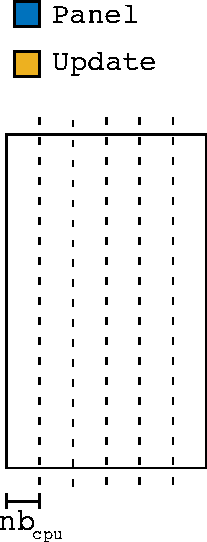
\includegraphics[width=0.8\textwidth]{figures/front_part_fine}}%
        \only<2>{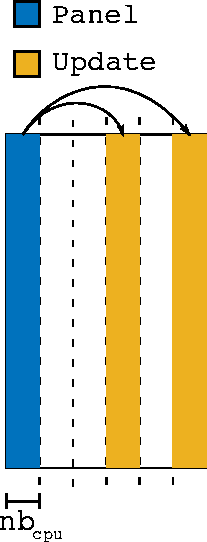
\includegraphics[width=0.8\textwidth]{figures/front_part_fine_ops}}%
        \only<3>{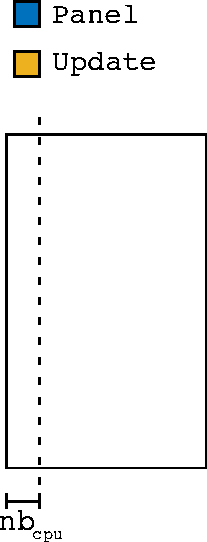
\includegraphics[width=0.8\textwidth]{figures/front_part_coarse}}%
        \only<4>{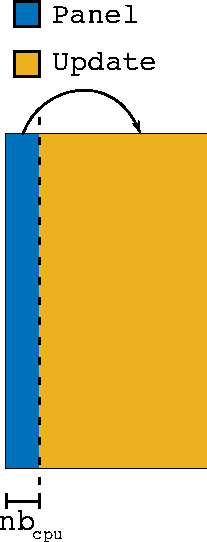
\includegraphics[width=0.8\textwidth]{figures/front_part_coarse_ops}}%
        \only<5>{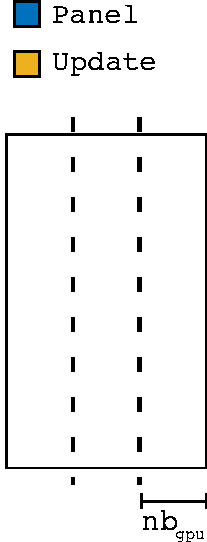
\includegraphics[width=0.8\textwidth]{figures/front_part_hier}}%
        \only<6>{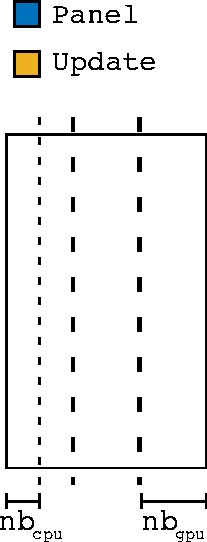
\includegraphics[width=0.8\textwidth]{figures/front_part_hier_repart}}%
        \only<7->{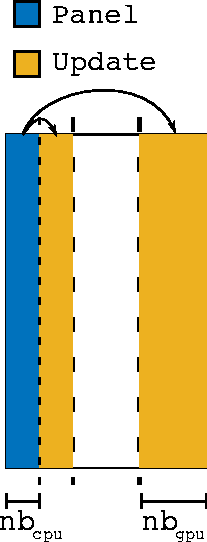
\includegraphics[width=0.8\textwidth]{figures/front_part_hier_ops}}
      \end{center}
    \end{column}
  \end{columns}
\end{frame}

\begin{frame}[fragile]{Frontal matrices partitioning strategies}

% The partitioning is achieved \alert{dynamically} through a
% partitioning task:

\begin{itemize}
% \item the partitioning is dynamic
\item The partitioning is done \alert{dynamically} through a
  \alert{partitioning task}.
\item the partitioning is \alert{symbolic}: neither allocations nor data
  copies.
\item the runtime ensures the \alert{consistency} of data.
\end{itemize}
  
\vspace{0.5cm}

\lstinputlisting[escapechar=|]{listings/hierarchical.f90}


% \begin{lstlisting}[basicstyle=\tt\tiny]
% forall outer panels o_p=1...o_n in f
%    ! partition (outer) block column f(o_p) into
%    ! i_n inner block columns f(o_p,1) .. f(o_p,i_n)
%    call submit(partition, f(o_p):R, f(o_p,1):RW, .., f(o_p,i_n):RW)

%    forall inner panels i_p=1..i_n
%       ! panel reduction of inner block column i_p
%       call submit(inner_panel, f(i_p):RW)
%       forall inner blockcolumns i_u=i_p+1..i_n in f(o_p)
%         ! update (inner) column in_u with panel p
%         call submit(inner_update, f(i_p):R, f(i_u):RW)
%       end do
%    end do

%    forall outer blockcolumns o_u=o_p+1..o_n
%       forall inner panels i_p=1..in_n
%        ! update outer block column o_u with panel i_p
%          call submit(outer_update, f(i_p):R,f(o_u):RW)
%       end do
%    end do     

%    ! unpartition (outer) block column
%    call submit(unpartition, f(o_p,1):R..f(o_p,i_n):R, f(o_p):RW)
% end do
%   \end{lstlisting}

\end{frame}

\begin{frame}{Tasks scheduling for heterogeneous architecture}

  % Multiple sources of heterogeneity:

  % \begin{columns}
  %   \begin{column}{0.5\textwidth}

  \begin{block}{Workload heterogeneity}
    \begin{itemize}
    \item \alert{Hierarchical partitioning}: fine and coarse
      granularity tasks.
    \item \alert{Variability of front sizes}: variation of tasks
      granularity.
    \item \dr{Compute-bound} and \dr{memory-bound} tasks.
    \end{itemize}    
  \end{block}

  % \end{column}
  % \begin{column}{0.5\textwidth}

  \begin{block}{Architecture heterogeneity}
    \begin{itemize}
    \item \dr{Processor} speeds and capabilities.
    \item \dr{Memory} speeds and transfers.
    \end{itemize}
  \end{block}

  % \end{column}
  % \end{columns}

  % \begin{itemize}
  %   \item Workload heterogeneity:
  %     \begin{itemize}
  %     \item The \alert{hierarchical partitioning} scheme produces fine and
  %       coarse granularity tasks.
  %     \item The \alert{variability of front sizes} in the etree induces a big
  %       variation of tasks granularity.
  %     \item Compute-bound and memory-bound tasks.
  %     \end{itemize}
  %   \item Architecture heterogeneity:
  %     \begin{itemize}
  %     \item Processor speeds.
  %     \item Memory speeds.
  %     \item Memory transfers.
  %     \end{itemize}
  % \end{itemize}

  \vspace{0.5cm}

  \dr{Multiple sources of heterogeneity}: Efficiently execute the task
  graph on the architecture requires a clever \alert{scheduling}
  strategy capable of taking into account resource capabilities.
 
\end{frame}

\begin{frame}[t]{Dynamic scheduling: building blocks}
  
  \vspace{-0.5cm}

  \begin{center}
    \only<1>{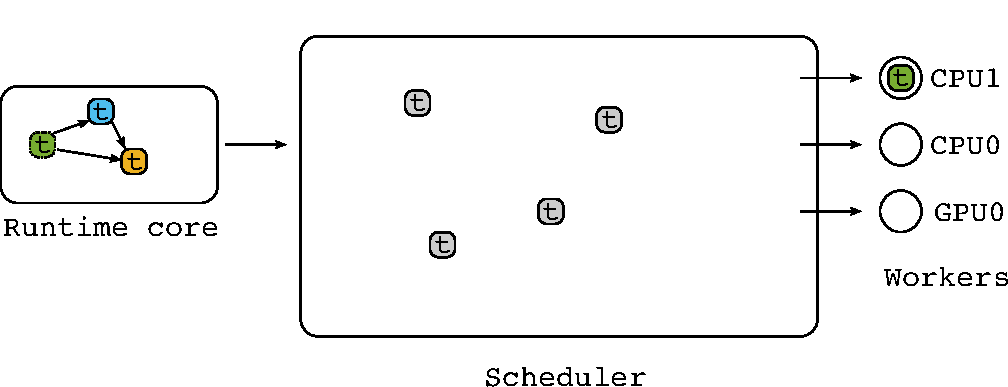
\includegraphics[width=0.8\textwidth]{figures/sched_running}}%
    \only<2>{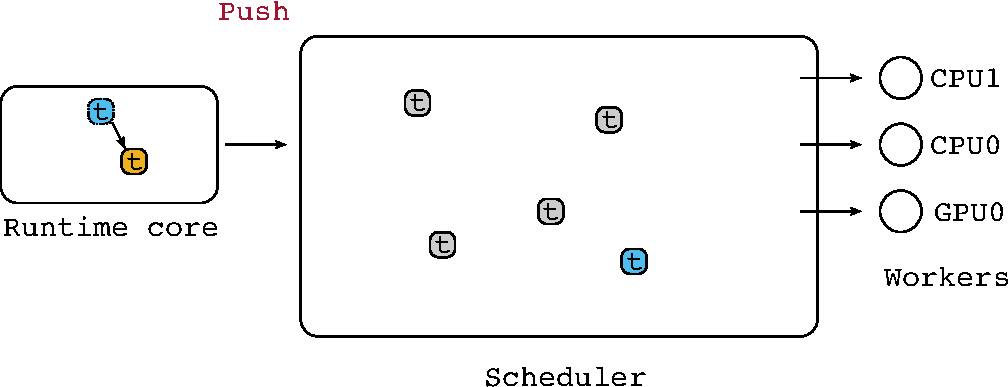
\includegraphics[width=0.8\textwidth]{figures/sched_push}}%
    \only<3>{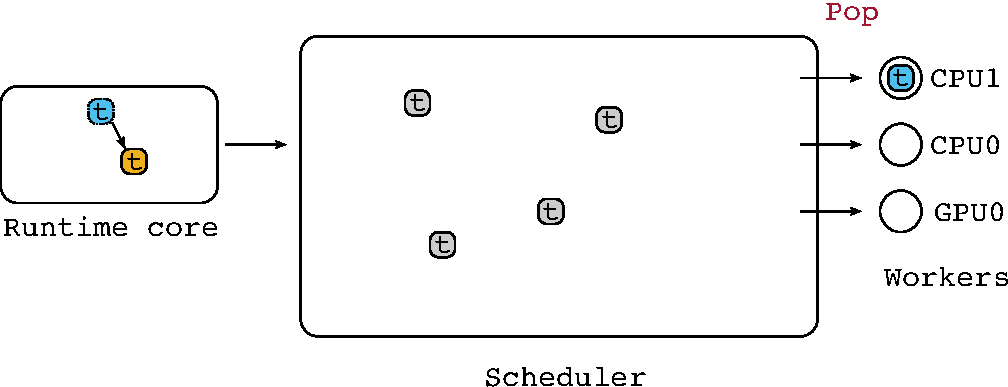
\includegraphics[width=0.8\textwidth]{figures/sched_pop}}%
    % \only<4-5>{\includegraphics[width=0.8\textwidth]{figures/sched_heft}}%
  \end{center}

  \vspace{-0.5cm}

  \begin{overlayarea}{\textwidth}{4cm}
    \only<1-3>{%
      \begin{block}{Building Blocks}
        \begin{itemize}
        \item A \dr{task container} storing tasks ready for execution.
        \item<2-3> Two methods:
          \begin{itemize}
          \item<2-3> \dr{{\tt push}}: put ready tasks in the scheduler.
          \item<3> \dr{{\tt pop }}: retrieve ready tasks from scheduler.
          \end{itemize}
        \end{itemize}
      \end{block}}%
    % \only<4-5>{%
    %   \begin{block}{DMDA (dynamic variant of HEFT~\cite{t.h.w:02})}
    %     \begin{itemize}
    %     \item<4-5> One queue per worker
    %     \item<4-5> Tasks are assigned at {\tt push} according to task priorities and a
    %       \alert{Minimum Completion Time} criterion
    %     \item[\dg{$\blacktriangle$}]<5> Data prefetching
    %     \item[\dr{$\blacktriangledown$}]<5> Runtime overhead: centralized and expensive 
    %     \item[\dr{$\blacktriangledown$}]<5> Local decision                              
    %     \end{itemize}
    %   \end{block}}%
  \end{overlayarea}
\end{frame}

\begin{frame}[t]{HeteroPrio scheduler}
  
  \vspace{-0.5cm}

  \begin{center}
    \only<1->{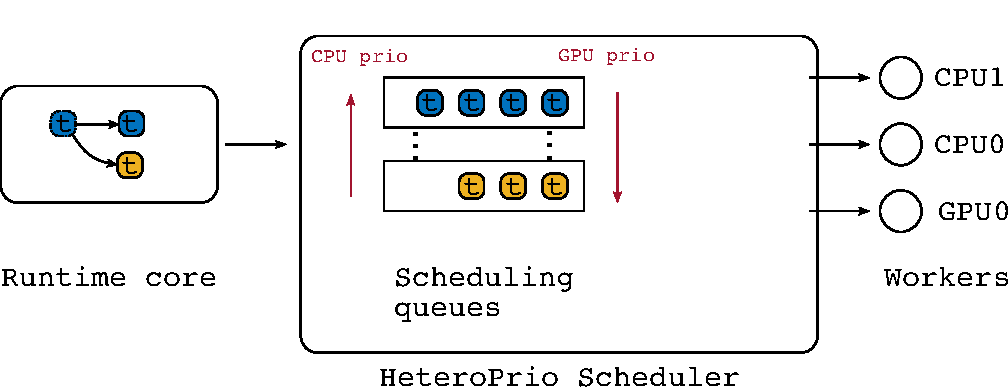
\includegraphics[width=0.8\textwidth]{figures/sched_hp}}%
  \end{center}

  \vspace{-0.5cm}

  \begin{block}{HeteroPrio}
    \begin{itemize}
    \item Introduced by Agullo \textit{et al.} for Fast Multipole Methods;
    \item Tasks are prioritized on each type of resources
      according to their \dr{acceleration factor}:
      \begin{enumerate}
      \item Performance ratio compared to other resources;
      \item Kernel efficiency.
      \end{enumerate}
    \item[\dg{$\blacktriangle$}]<2> Good matching between tasks
      and units.
    \end{itemize}
  \end{block}
\end{frame}

\begin{frame}[t]{HeteroPrio scheduler: extension 1/2}
  
  \vspace{-0.5cm}

  \begin{center}
    % \only<1>{\includegraphics[width=0.8\textwidth]{sched_hp_steady}}%
    \only<1->{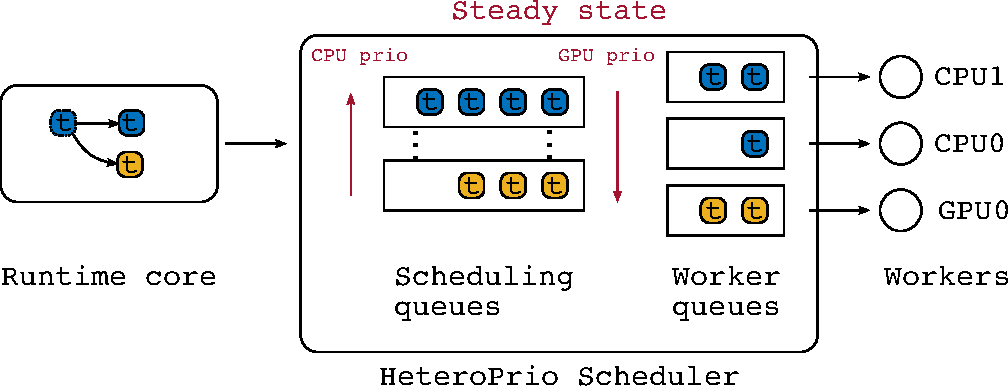
\includegraphics[width=0.8\textwidth]{figures/sched_hp_steady_wqueues}}%
  \end{center}

  \vspace{-0.5cm}

  \begin{overlayarea}{\textwidth}{4cm}
    \only<1-2>{%
      \begin{block}{HeteroPrio: data prefetching}
        \begin{itemize}
        \item Added one worker queue per worker;
        \item Tasks are put in scheduling queues at \dr{push}
          operation and moved to worker queues at \dr{pop};
        \item[\dg{$\blacktriangle$}]<2> Slightly anticipated task
          assignment: overlapped communication and computations.
        \end{itemize}
      \end{block}}%
  \end{overlayarea}
\end{frame}

\begin{frame}[t]{HeteroPrio scheduler: extension 2/2}

  % The scheduler HeteroPrio is introducted in~\citet{a.b.c.d.ea:14} in
  % the context of Fast Multipole methods.

  \begin{center}
    \only<1>{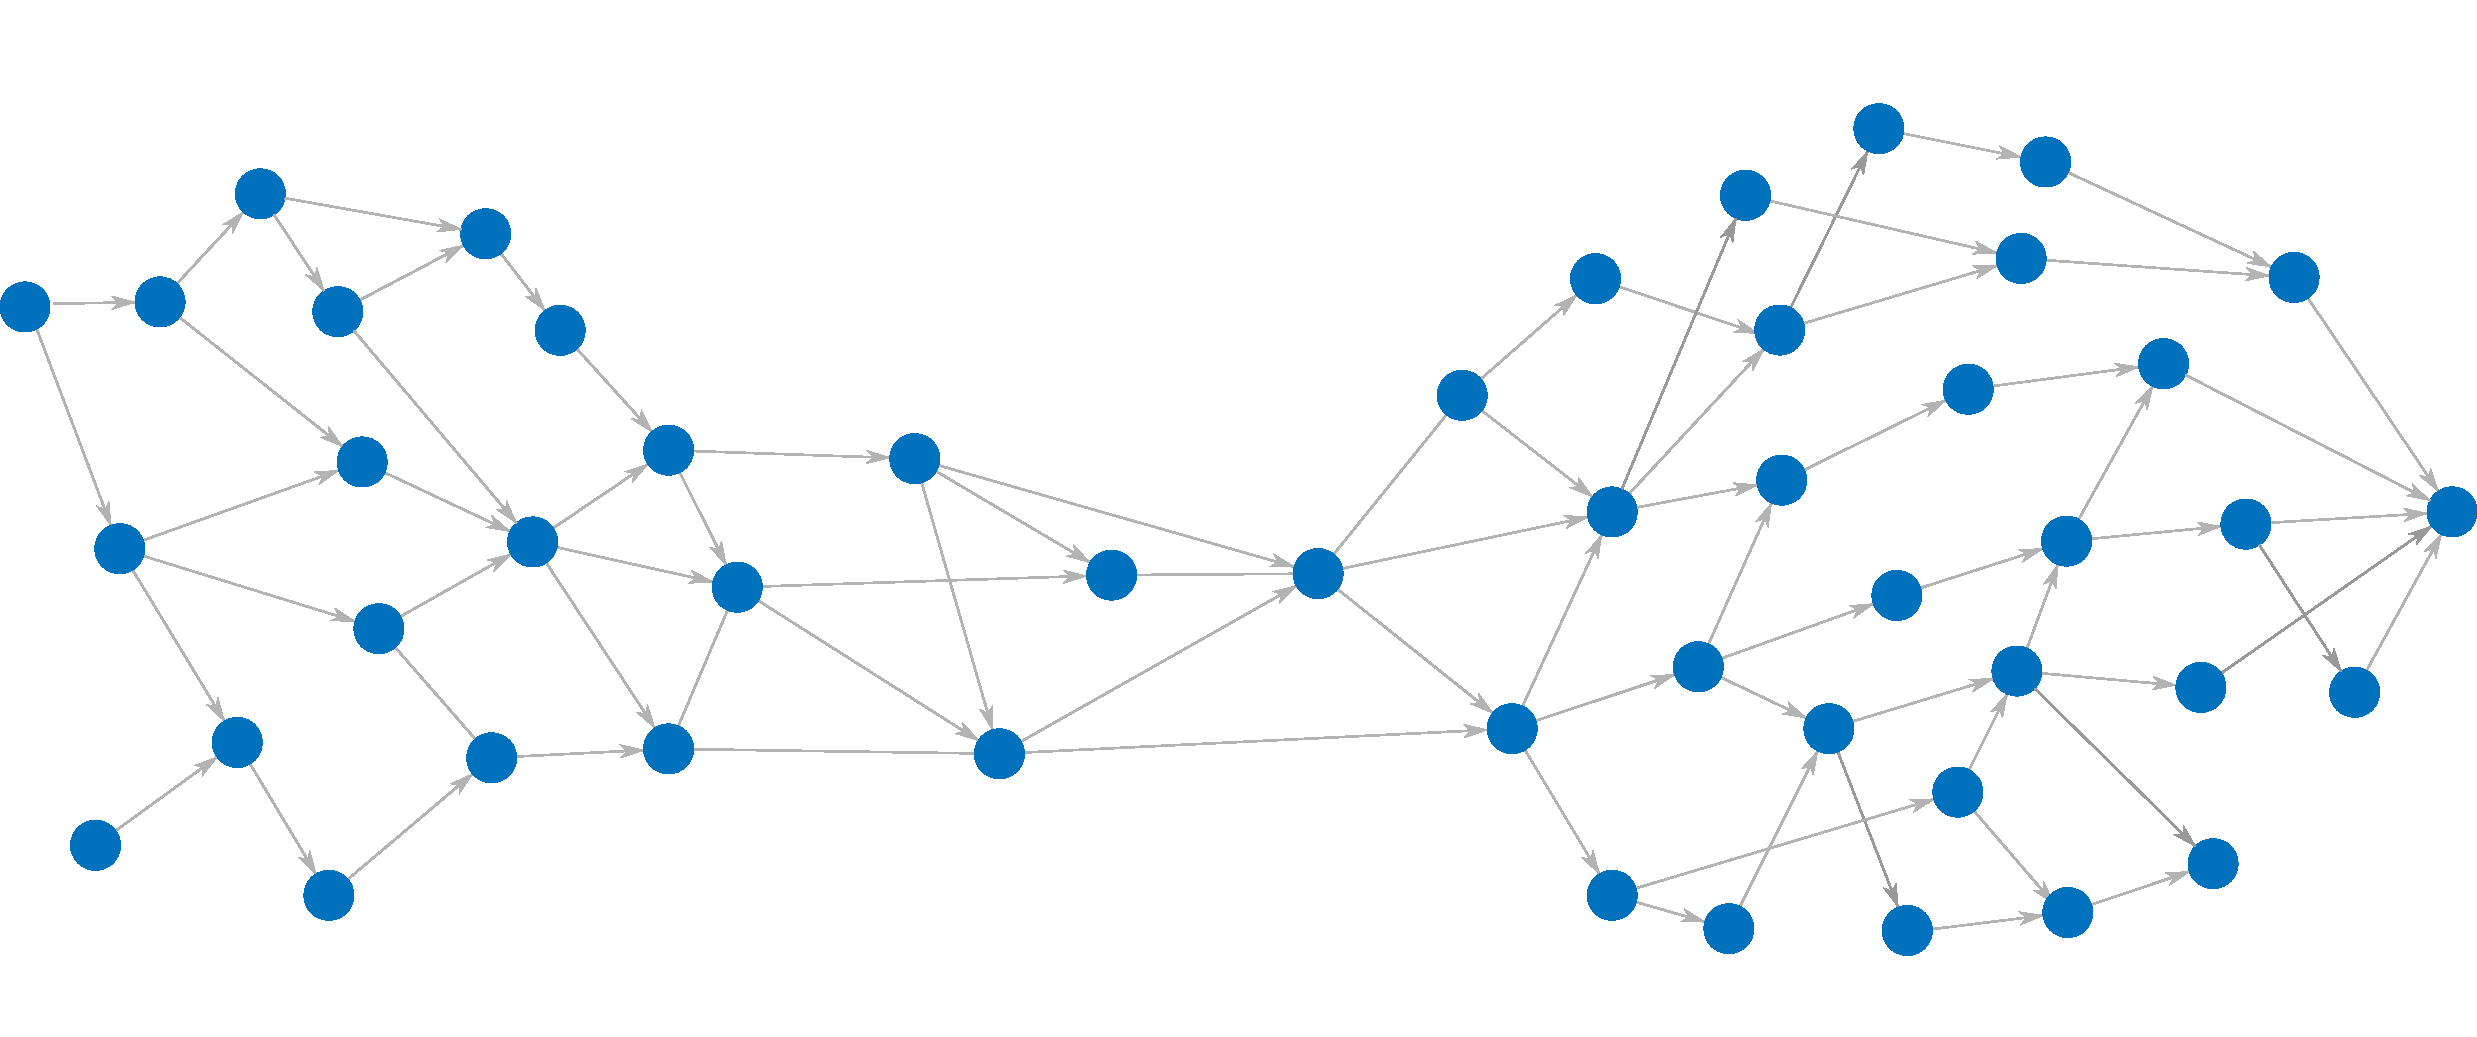
\includegraphics[width=0.8\textwidth]{figures/irregular_dag1}}%
    \only<2>{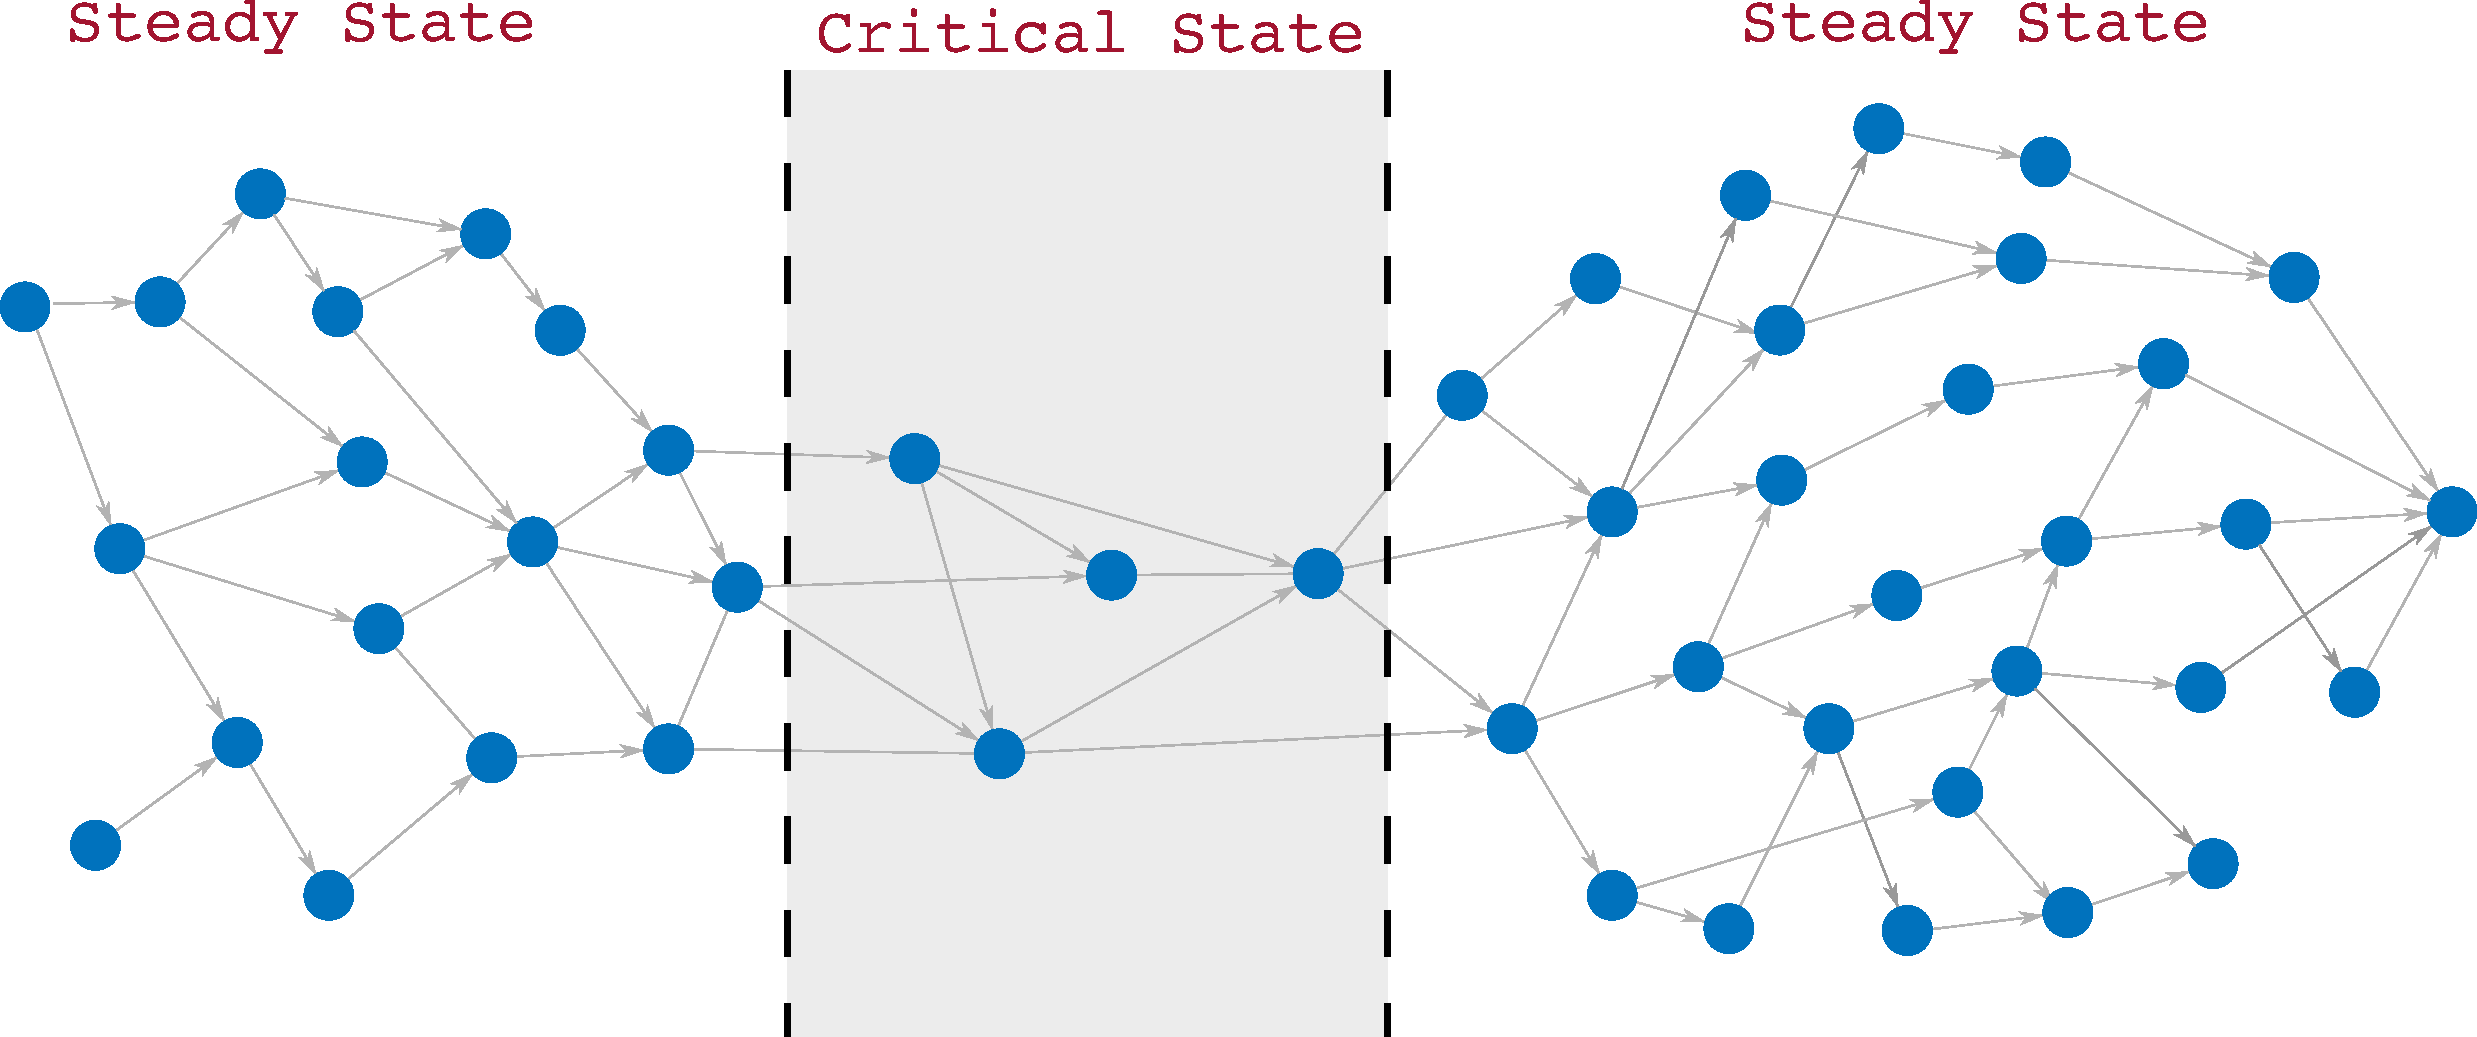
\includegraphics[width=0.8\textwidth]{figures/irregular_dag2}}%
  \end{center}

  % The parallel execution consists in a succession of two states:
  DAGs may be irregular and alternate rich and poor concurrency
  regions. \uncover<2>{
  Our scheduler switches automatically between two states:
  \begin{itemize}
  \item \db{Steady-state}: \# of ready tasks $>>$ number of resources:
    \alert{execute tasks where they are best suited} i.e. best
    acceleration factor.
  \item \db{Critical-state}: \# of ready tasks $<<$ number of resources:
    \alert{reduce the time spent on the critical path}.
  \end{itemize}}

  % \begin{center}
  %   \includegraphics[width=0.8\textwidth]{figures/steady_critical}
  % \end{center}

  % We use two set of queues: scheduling and worker queues and
  % scheduling decisions are taken at \alert{ {\tt pop}} operation:
  % \begin{itemize}
  % \item Pull a task form worker queue.
  % \item Fill worker queue retrieving tasks from scheduling queue.
  % \end{itemize}
\end{frame}

\begin{frame}[t]{HeteroPrio scheduler: extension 2/2}
    
  \begin{center}
    \only<1>{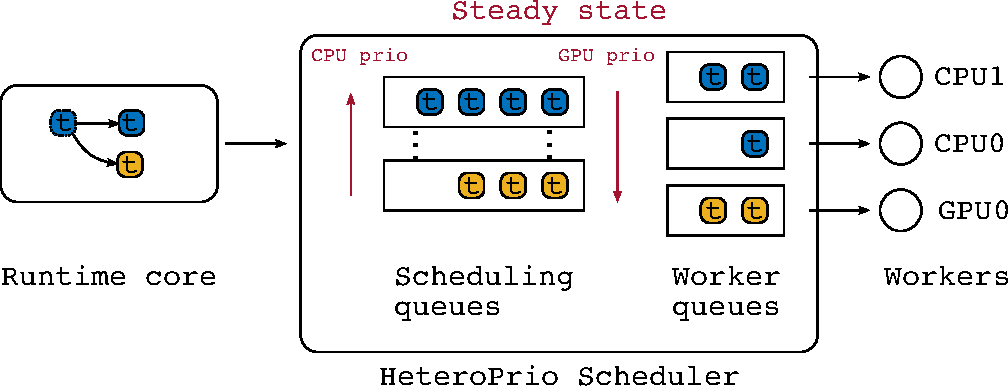
\includegraphics[width=0.8\textwidth]{figures/sched_hp_steady_wqueues}}%
    \only<2->{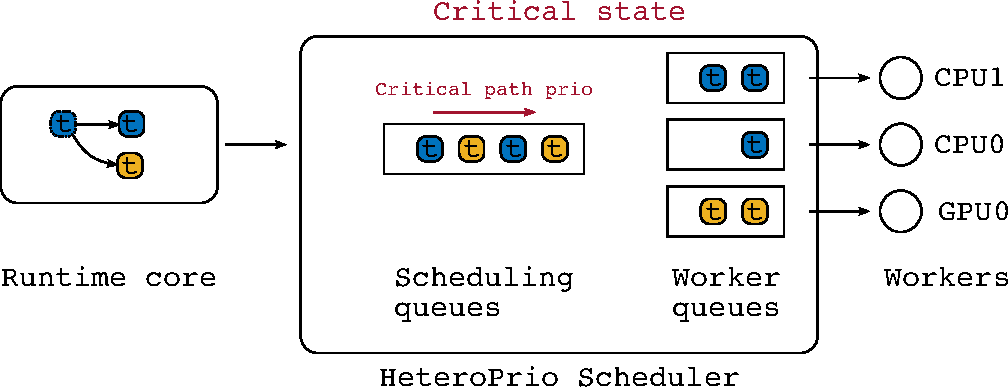
\includegraphics[width=0.8\textwidth]{figures/sched_hp_critical}}%
  \end{center}

  % \vspace{-0.5cm}

  \begin{block}{HeteroPrio: dynamic policy switching}
    \begin{itemize}
    \item<1-> \dr{Steady-state}: high concurrency $\Rightarrow$ maximize tasks acceleration
      \begin{itemize}
      \item[\dg{$\blacktriangle$}]<1-> Good matching between tasks
      and units. 
      \end{itemize}
    \item<2-> \dr{Critical-state}: low concurrency $\Rightarrow$ improve the critical path          
      \begin{itemize}
      \item[\dg{$\blacktriangle$}]<2-> Avoid stalls in the pipeline. 
      \end{itemize}
    \end{itemize}
  \end{block}
\end{frame}

\begin{frame}{Experimental results}
  \centering
  \texttt{\small
    \begin{tabular}{rlrl}
      \hline
      \# & Matrix          & Gflops & Ordering \\
      \hline
      12 & hirlam          & 1384   & SCOTCH   \\
      13 & flower\_8\_4    & 2851   & SCOTCH   \\
      14 & Rucci1          & 5671   & SCOTCH   \\
      15 & ch8-8-b3        & 10709  & SCOTCH   \\
      16 & GL7d24          & 16468  & SCOTCH   \\
      17 & neos2           & 20170  & SCOTCH   \\
      18 & spal\_004       & 30336  & SCOTCH   \\
      19 & n4c6-b6         & 62246  & SCOTCH   \\
      21 & TF18            & 194473 & SCOTCH   \\      
      \hline
      2  & karted          & 279    & COLAMD   \\
      5  & cat\_ears\_4\_4 & 786    & COLAMD   \\
      7  & e18             & 3399   & COLAMD   \\
      8  & flower\_7\_4    & 4261   & COLAMD   \\
      11 & TF17            & 38209  & COLAMD   \\
      24 & TF16            & 2884   & COLAMD   \\ 
      \hline
   \end{tabular}}
\end{frame}


\begin{frame}{Experimental results}
  {\bf System \db{Sirocco}} (Plafrim supercomputing center):

  \begin{columns}
    \begin{column}{0.5\textwidth}
      % \texttt{\tiny
      %   \begin{tabular}{rlrl}
      %     \hline
      %     \# & Matrix       & Mflops    & Ordering \\
      %     \hline
      %     12 & hirlam       & 1384160   & SCOTCH   \\
      %     13 & flower\_8\_4 & 2851508   & SCOTCH   \\
      %     14 & Rucci1       & 5671282   & SCOTCH   \\
      %     15 & ch8-8-b3     & 10709211  & SCOTCH   \\
      %     16 & GL7d24       & 16467844  & SCOTCH   \\
      %     17 & neos2        & 20170318  & SCOTCH   \\
      %     18 & spal\_004    & 30335566  & SCOTCH   \\
      %     19 & n4c6-b6      & 62245957  & SCOTCH   \\
      %     20 & sls          & 65607341  & SCOTCH   \\
      %     21 & TF18         & 194472820 & SCOTCH   \\
      %     22 & lp\_nug30    & 221644546 & SCOTCH   \\
      %     23 & mk13-b5      & 259751609 & SCOTCH   \\
      %     \hline
      %   \end{tabular}}

      
      \begin{itemize}
      \item Haswell Intel Xeon E5-2680 @ 2.5 GHz, $2\times 12$ cores
      \item 128 GB memory (NUMA)
      \item Nvidia K40 GPUs, 4 devices
      \end{itemize}

    \end{column}
    \begin{column}{0.5\textwidth}
        
        \begin{itemize}
        \item Compilers Intel ifort and icc 15.0.2
        \item BLAS and LAPACK libraries from Intel MKL 11.2.
        \end{itemize}
    \end{column}
  \end{columns}

  \begin{center}
    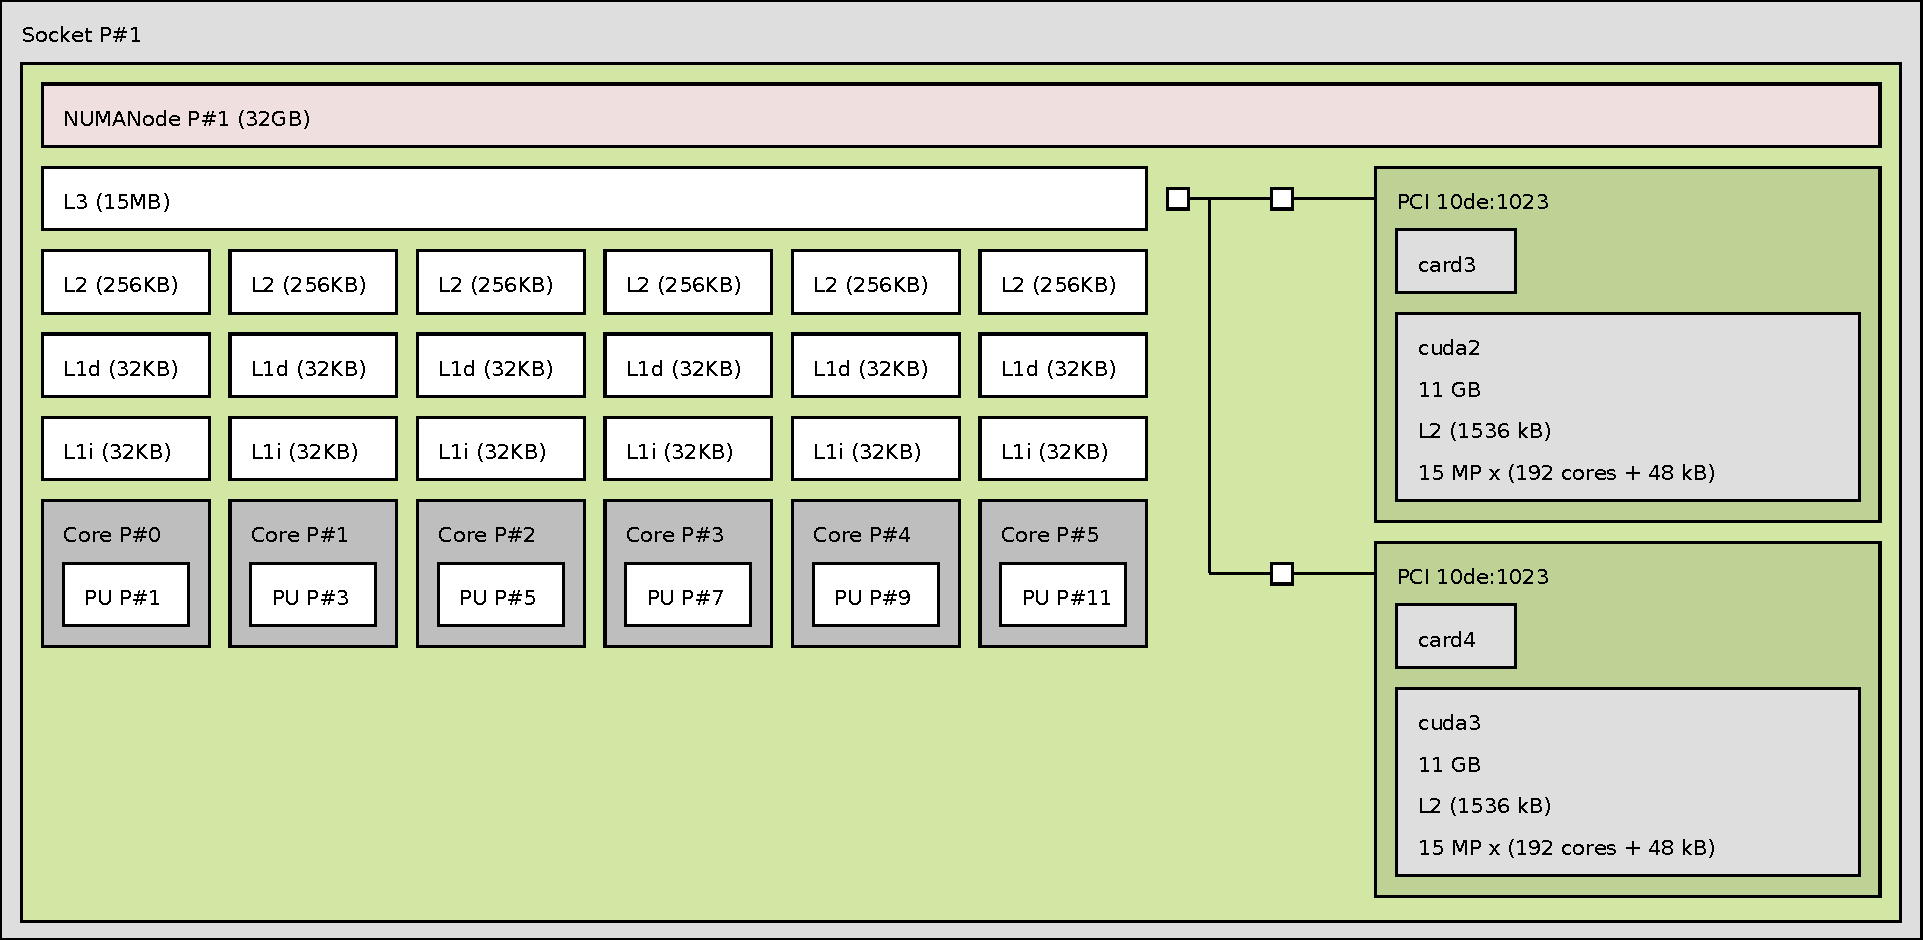
\includegraphics[width=0.8\textwidth]{figures/sirocco2}
  \end{center}

\end{frame}

\begin{frame}{Experimental results: absolute performance}
  \centering
  \only<1>{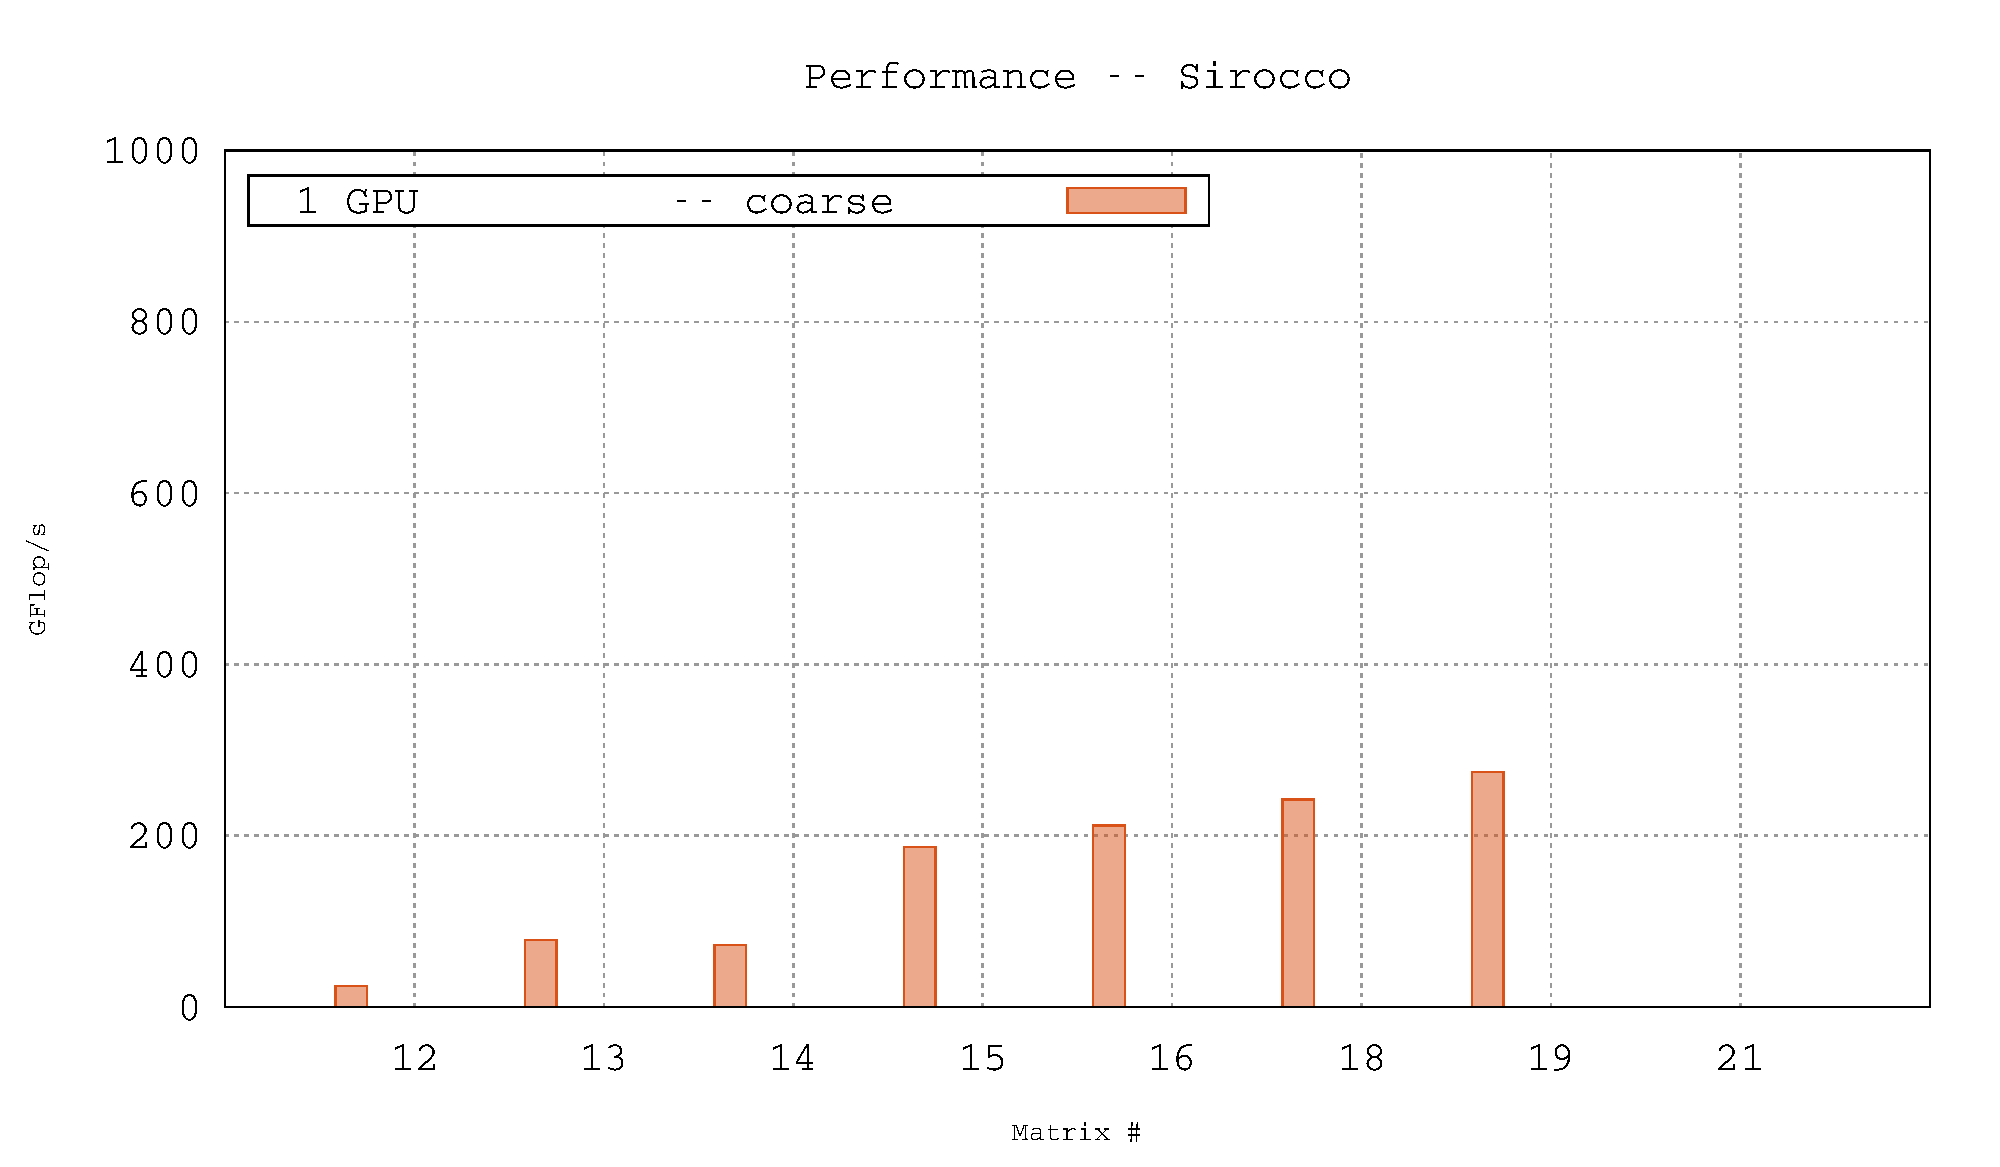
\includegraphics[width=\textwidth]{figures/perf_sirocco2_1}}%
  \only<2>{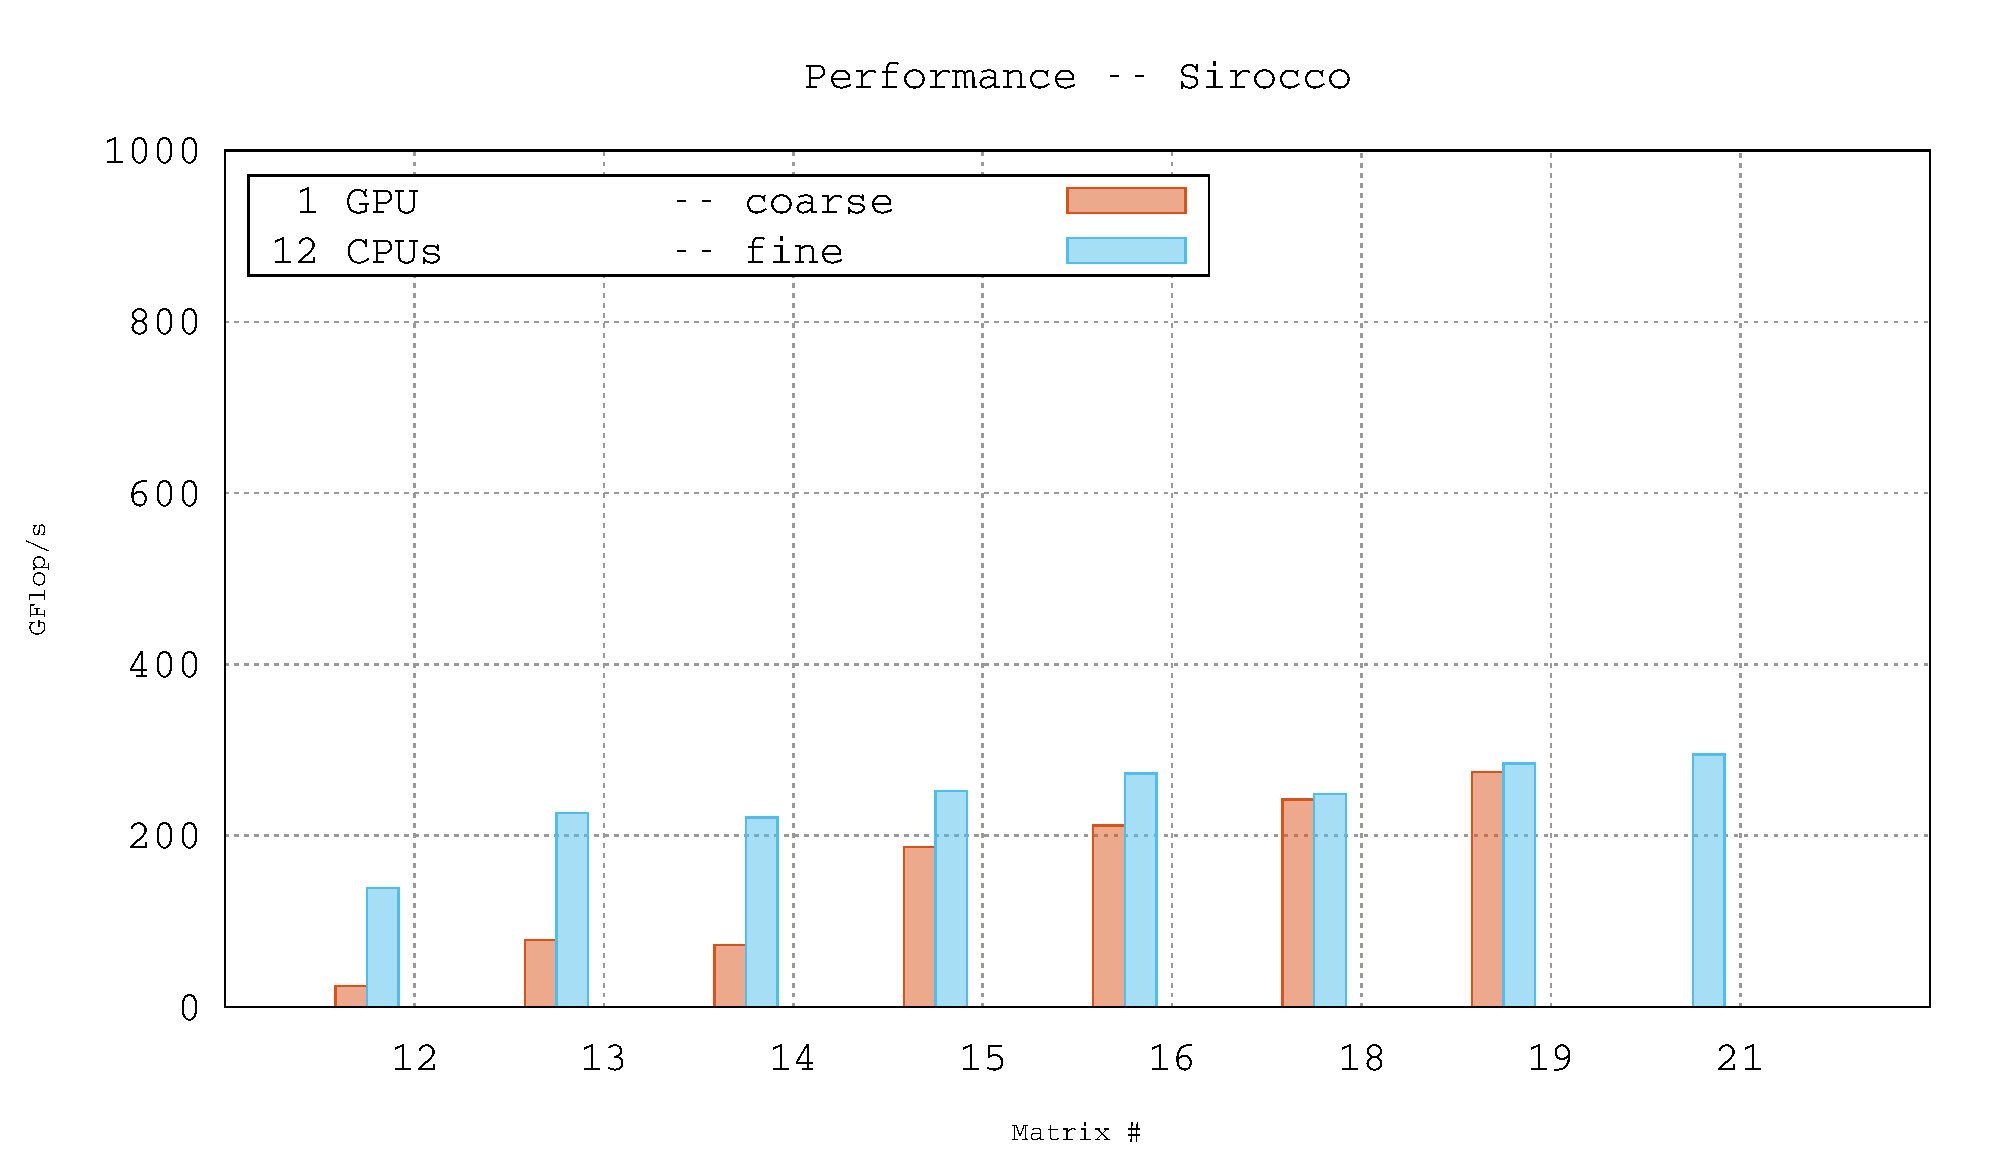
\includegraphics[width=\textwidth]{figures/perf_sirocco2_2}}%
  \only<3>{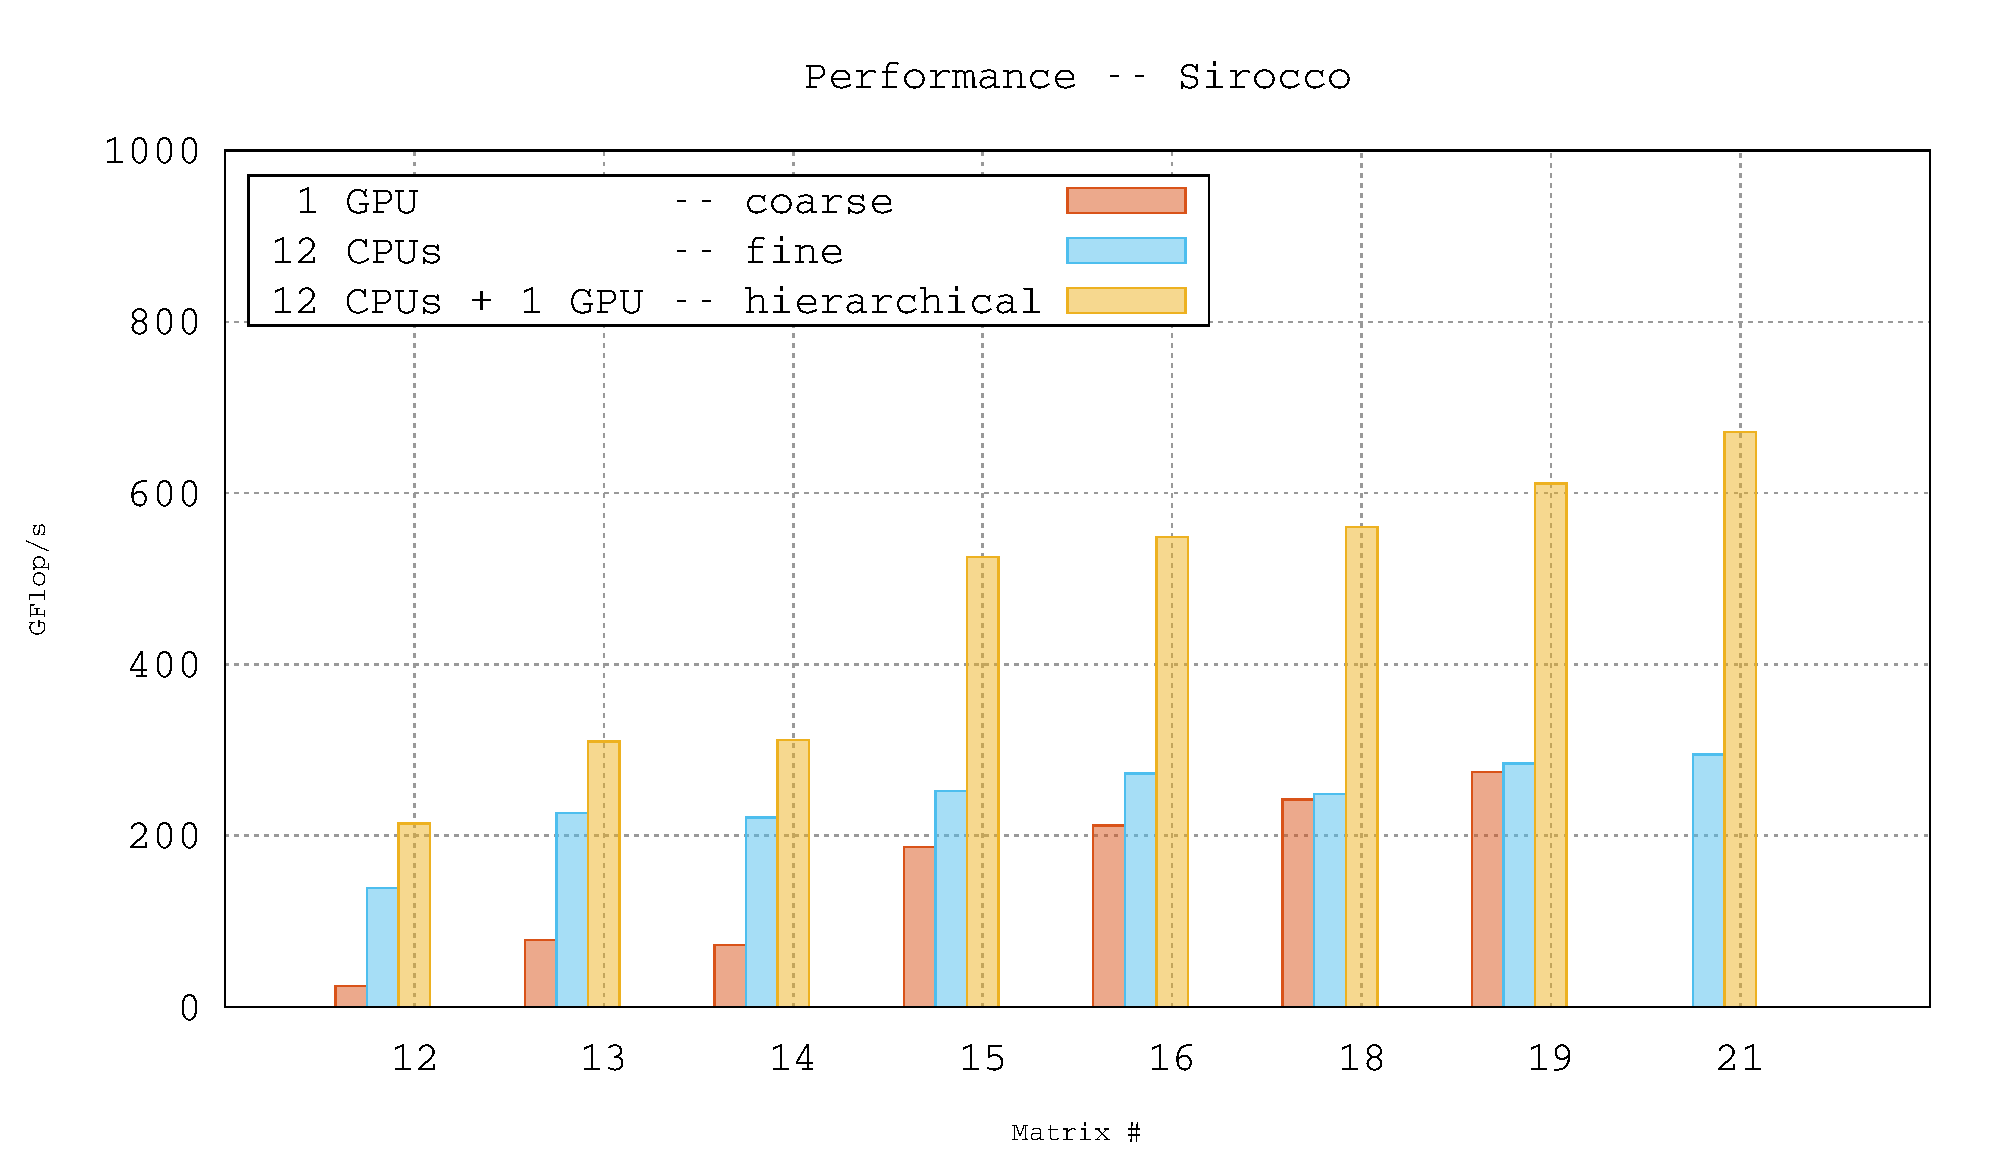
\includegraphics[width=\textwidth]{figures/perf_sirocco2_3}}%
  \only<4>{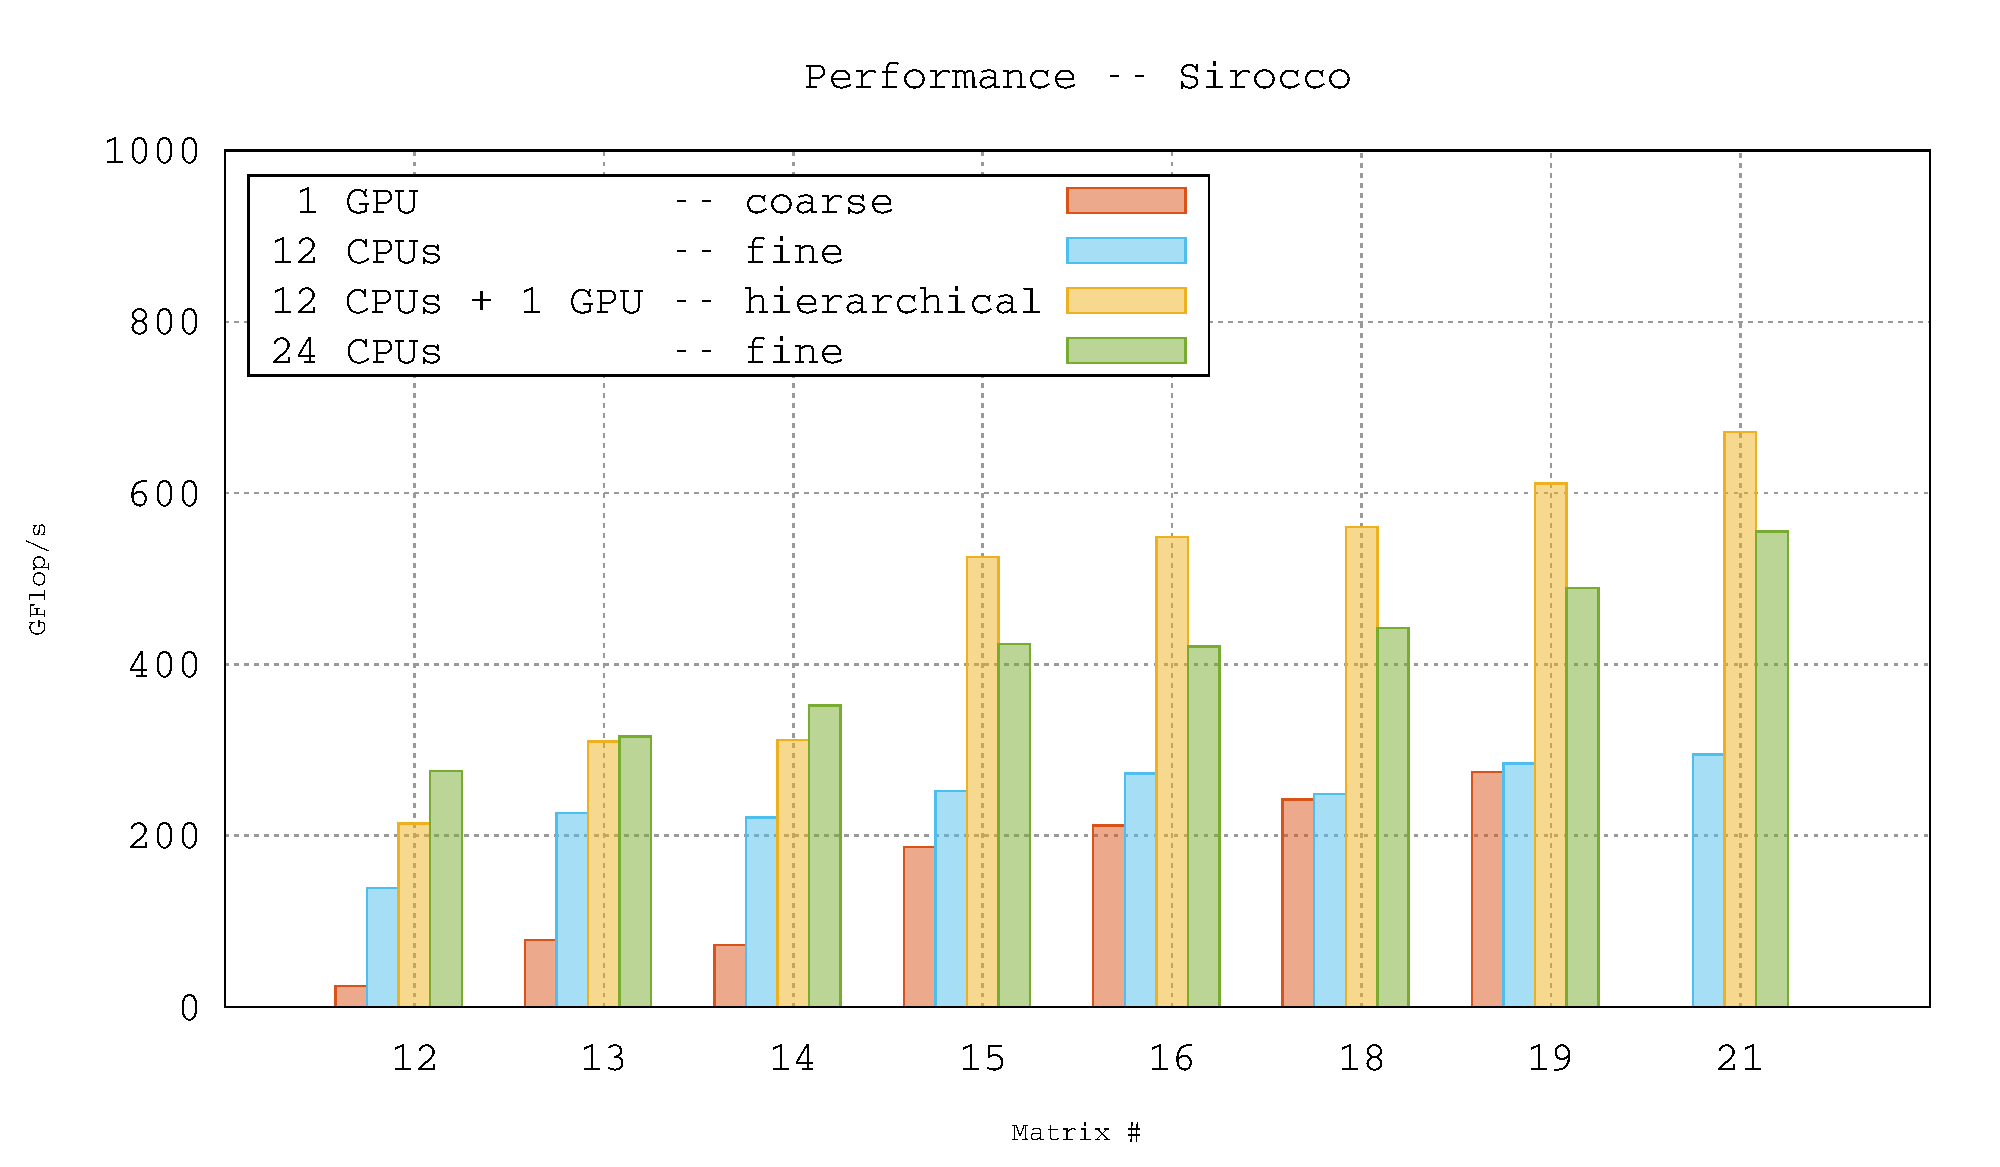
\includegraphics[width=\textwidth]{figures/perf_sirocco2_4}}%
  \only<5>{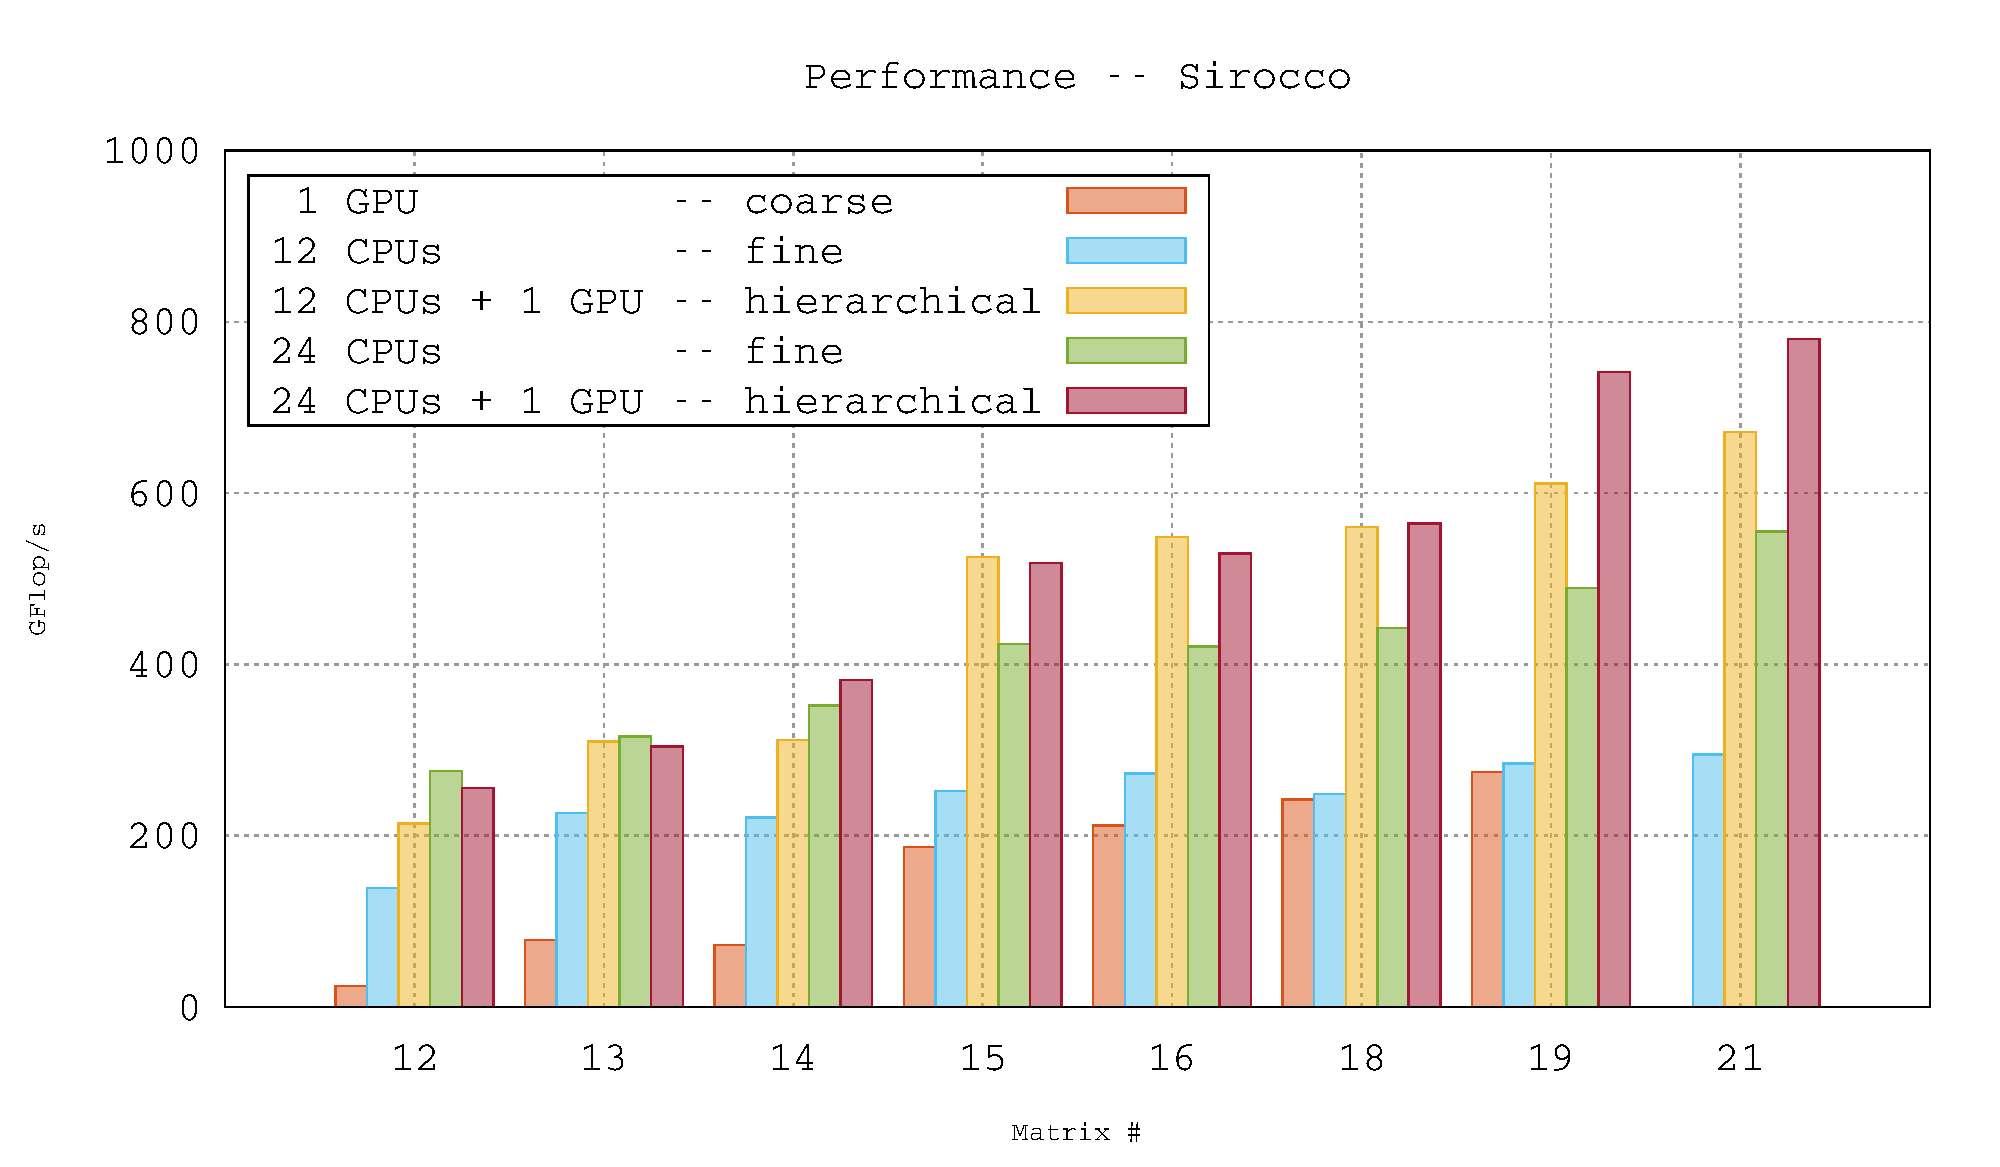
\includegraphics[width=\textwidth]{figures/perf_sirocco2}}%
\end{frame}

\begin{frame}{Area performance upper bound}

  The parallel efficiency can be defined as

  \begin{displaymath}
    e(p) = \frac{t^{min}(p)}{t(p)}
  \end{displaymath}

  where \dr{$t^{min}(p)$} is a lower bound on execution time on $p$
  resources corresponding to the \alert{best schedule} under the
  following assumptions:

  \begin{columns}
    \begin{column}{0.45\textwidth}

      \begin{enumerate}
      \item<2-> No runtime overhead and no communications.
      \item<3-> No tasks dependencies.
      \item<4-> Tasks are moldable.

        %% \item<2-> Tasks executed at asymptotic performance (\alert{maximum task granularity})
        %% \item<2-> \alert{Perfect data locality}
      \end{enumerate}

    \end{column}
    \begin{column}{0.55\textwidth}

      \begin{center}
        \only<1>{\includegraphics[width=\textwidth]{figures/lp_anim2}}%
        \only<2>{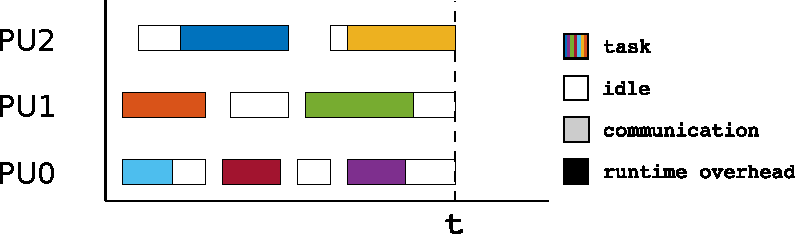
\includegraphics[width=\textwidth]{figures/lp_anim3}}%
        \only<3>{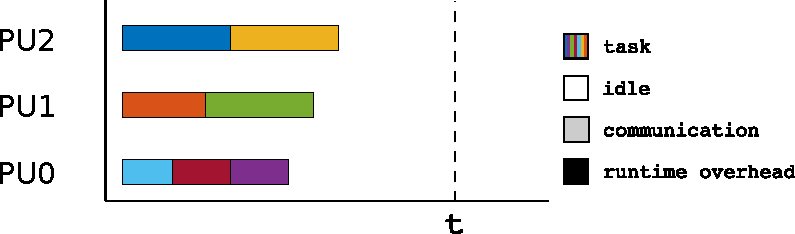
\includegraphics[width=\textwidth]{figures/lp_anim4}}%
        \only<4->{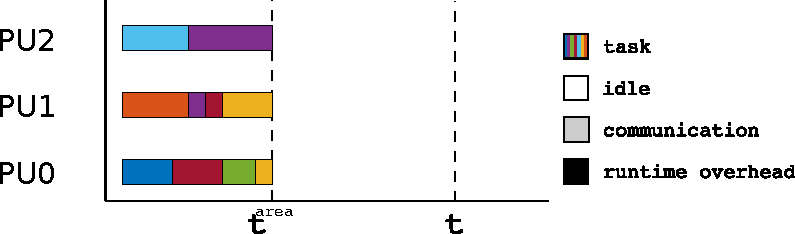
\includegraphics[width=\textwidth]{figures/lp_anim5}}%

        % \only<2>{\includegraphics[width=\textwidth]{lp_anim2}}%
      \end{center}

    \end{column}
  \end{columns}
  
  \vspace{1cm}

  \begin{overlayarea}{\textwidth}{2cm}

    \only<5>{In the heterogeneous case we have $t^{area}(p)$ is the
      solution of a \dr{linear program}.}%
    
    \only<6->{We consider \dr{$t^{area}(p)$} when there is no
      performance loss resulting from the parallelization:
      \dr{$\tilde{t}^{area}(p)$}.}%

  \end{overlayarea}

\end{frame}

\begin{frame}{A finer performance analysis}
  The execution time $t(p)$ can be decomposed in the following four
  terms:
  \begin{itemize}
  \item<1-> \db{$t_t(p)$}: the time spent executing tasks.
  \item<1-> \mye{$t_r(p)$}: the overhead of the runtime system.
  \item<1-> \dg{$t_i(p)$}: idle time.
  \item<2-> \mbp{$t_c(p)$}: the time spent performing communications.
  \end{itemize}

  The overall efficiency can thus be written as:
  
  {\tiny
\begin{align*}
  e(p) & = \frac{\tilde{t}^{area}(p)}{t(p)} =  \frac{\tilde{t}^{area}(p) \times p }{ t_t(p) + t_r(p) + t_c(p) + t_i(p) } = \frac{ \tilde{t}^{area}_t(p) }{ t_t(p) + t_r(p) + t_c(p) + t_i(p) } \\
  & =  \mre{\overbracket{\mbk{\frac{ \tilde{t}^{area}_t(p) }{ t^{area}_t(p) }}}^{e_g}}\cdot 
  \mbl{\overbracket{\mbk{\frac{ t^{area}_t(p) }{ t_t(p) }}}^{e_{t}}}\cdot  
  \mye{\overbracket{\mbk{\frac{ t_t(p) }{ t_t(p)+t_r(p) }}}^{e_r}}\cdot
  \uncover<2->{\mbp{\overbracket{\mbk{\frac{ t_t(p)+t_r(p) }{t_t(p)+t_r(p)+ t_c(p)}}}^{e_c}}\cdot}
  \mgr{\overbracket{\mbk{\frac{ t_t(p)+t_r(p)+ t_c(p) }{ t_t(p) + t_r(p) + t_c(p) + t_i(p) }}}^{e_p}}.
\end{align*}
 }
    % \begin{displaymath}
    %   \tiny
    %     e(p) = \mbk{\frac{\tilde{t}^{area}(p)}{t(p)}} 
    %     % = \frac{ \tilde{t}^{area}(p) \times p }{ t_t(p) + t_r(p) + t_c(p) + t_i(p) } = \frac{ \tilde{t}^{area}_t(p) }{ t_t(p) + t_r(p) + t_c(p) + t_i(p) }
    %     = \mre{\overbracket{\mbk{\frac{ \tilde{t}^{area}_t(p) }{ t^{area}_t(p) }}}^{e_g}}\cdot
    %     \mbl{\overbracket{\mbk{\frac{ t^{area}_t(p) }{ t_t(p) }}}^{e_{t}}}\cdot
    %     \mgr{\overbracket{\mbk{\frac{ t_t(p) }{ t_t(p)+t_r(p) }}}^{e_r}}\cdot
    %     \mbp{\overbracket{\mbk{\frac{ t_t(p)+t_r(p) }{t_t(p)+t_r(p)+ t_c(p)}}}^{e_c}}\cdot
    %     \mye{\overbracket{\mbk{\frac{ t_t(p)+t_r(p)+ t_c(p) }{ t_t(p) + t_r(p) + t_c(p) + t_i(p) }}}^{e_p}}.
    % \end{displaymath}

%   \begin{displaymath}
% e(p) = \frac{t^{area}(p)}{t(p)} =%
% \only<1,3,4,5>{\overbracket{\frac{t^{area}_t(p)}{t_t(p)}}^{e_h}}%
% \only<2>{\dr{\overbracket{\frac{t^{area}_t(p)}{t_t(p)}}^{e_h}}}%
% \cdot%
% \only<1,2,4,5>{\overbracket{\frac{t_t(p)}{t_t(p)+t_r(p)}}^{e_r}}%
% \only<3>{\dg{\overbracket{\frac{t_t(p)}{t_t(p)+t_r(p)}}^{e_r}}}%
% \cdot%
% \only<1,2,3,5>{\overbracket{\frac{t_t(p)+t_r(p)}{t_t(p)+t_r(p)+t_i(p)}}^{e_p}}%
% \only<4>{\db{\overbracket{\frac{t_t(p)+t_r(p)}{t_t(p)+t_r(p)+t_i(p)}}^{e_p}}}%
%   \end{displaymath}
  
  \vspace{0.5cm}

  with:

  \vspace{0.3cm}

  \begin{overlayarea}{\textwidth}{3cm}
    \only<2>{\mbp{$e_c$}: the \mbp{communication efficiency}. measures
      the cost of communications with respect to the actual work done
      due to data transfers between workers.}%

    \only<3>{\db{$e_t$}: the \db{task efficiency}. Measures how well
      the assignment of tasks to processing units matches the tasks
      properties to the units capabilities.}%

    % \begin{itemize}
    % \item<5> if $e_h>1$ GPUs are overloaded and CPU starve ($e_p<1$)
    % \item<5> if $e_h<1$ tasks acceleration factor not properly exploited
    % \end{itemize}%

    % \only<7>{$e_t \cdot e_p$ measures the quality of the scheduling
    % and is $\leq 1$.}
  \end{overlayarea}

\end{frame}

\begin{frame}{Experimental results: efficiency breakdown}
  \centering
  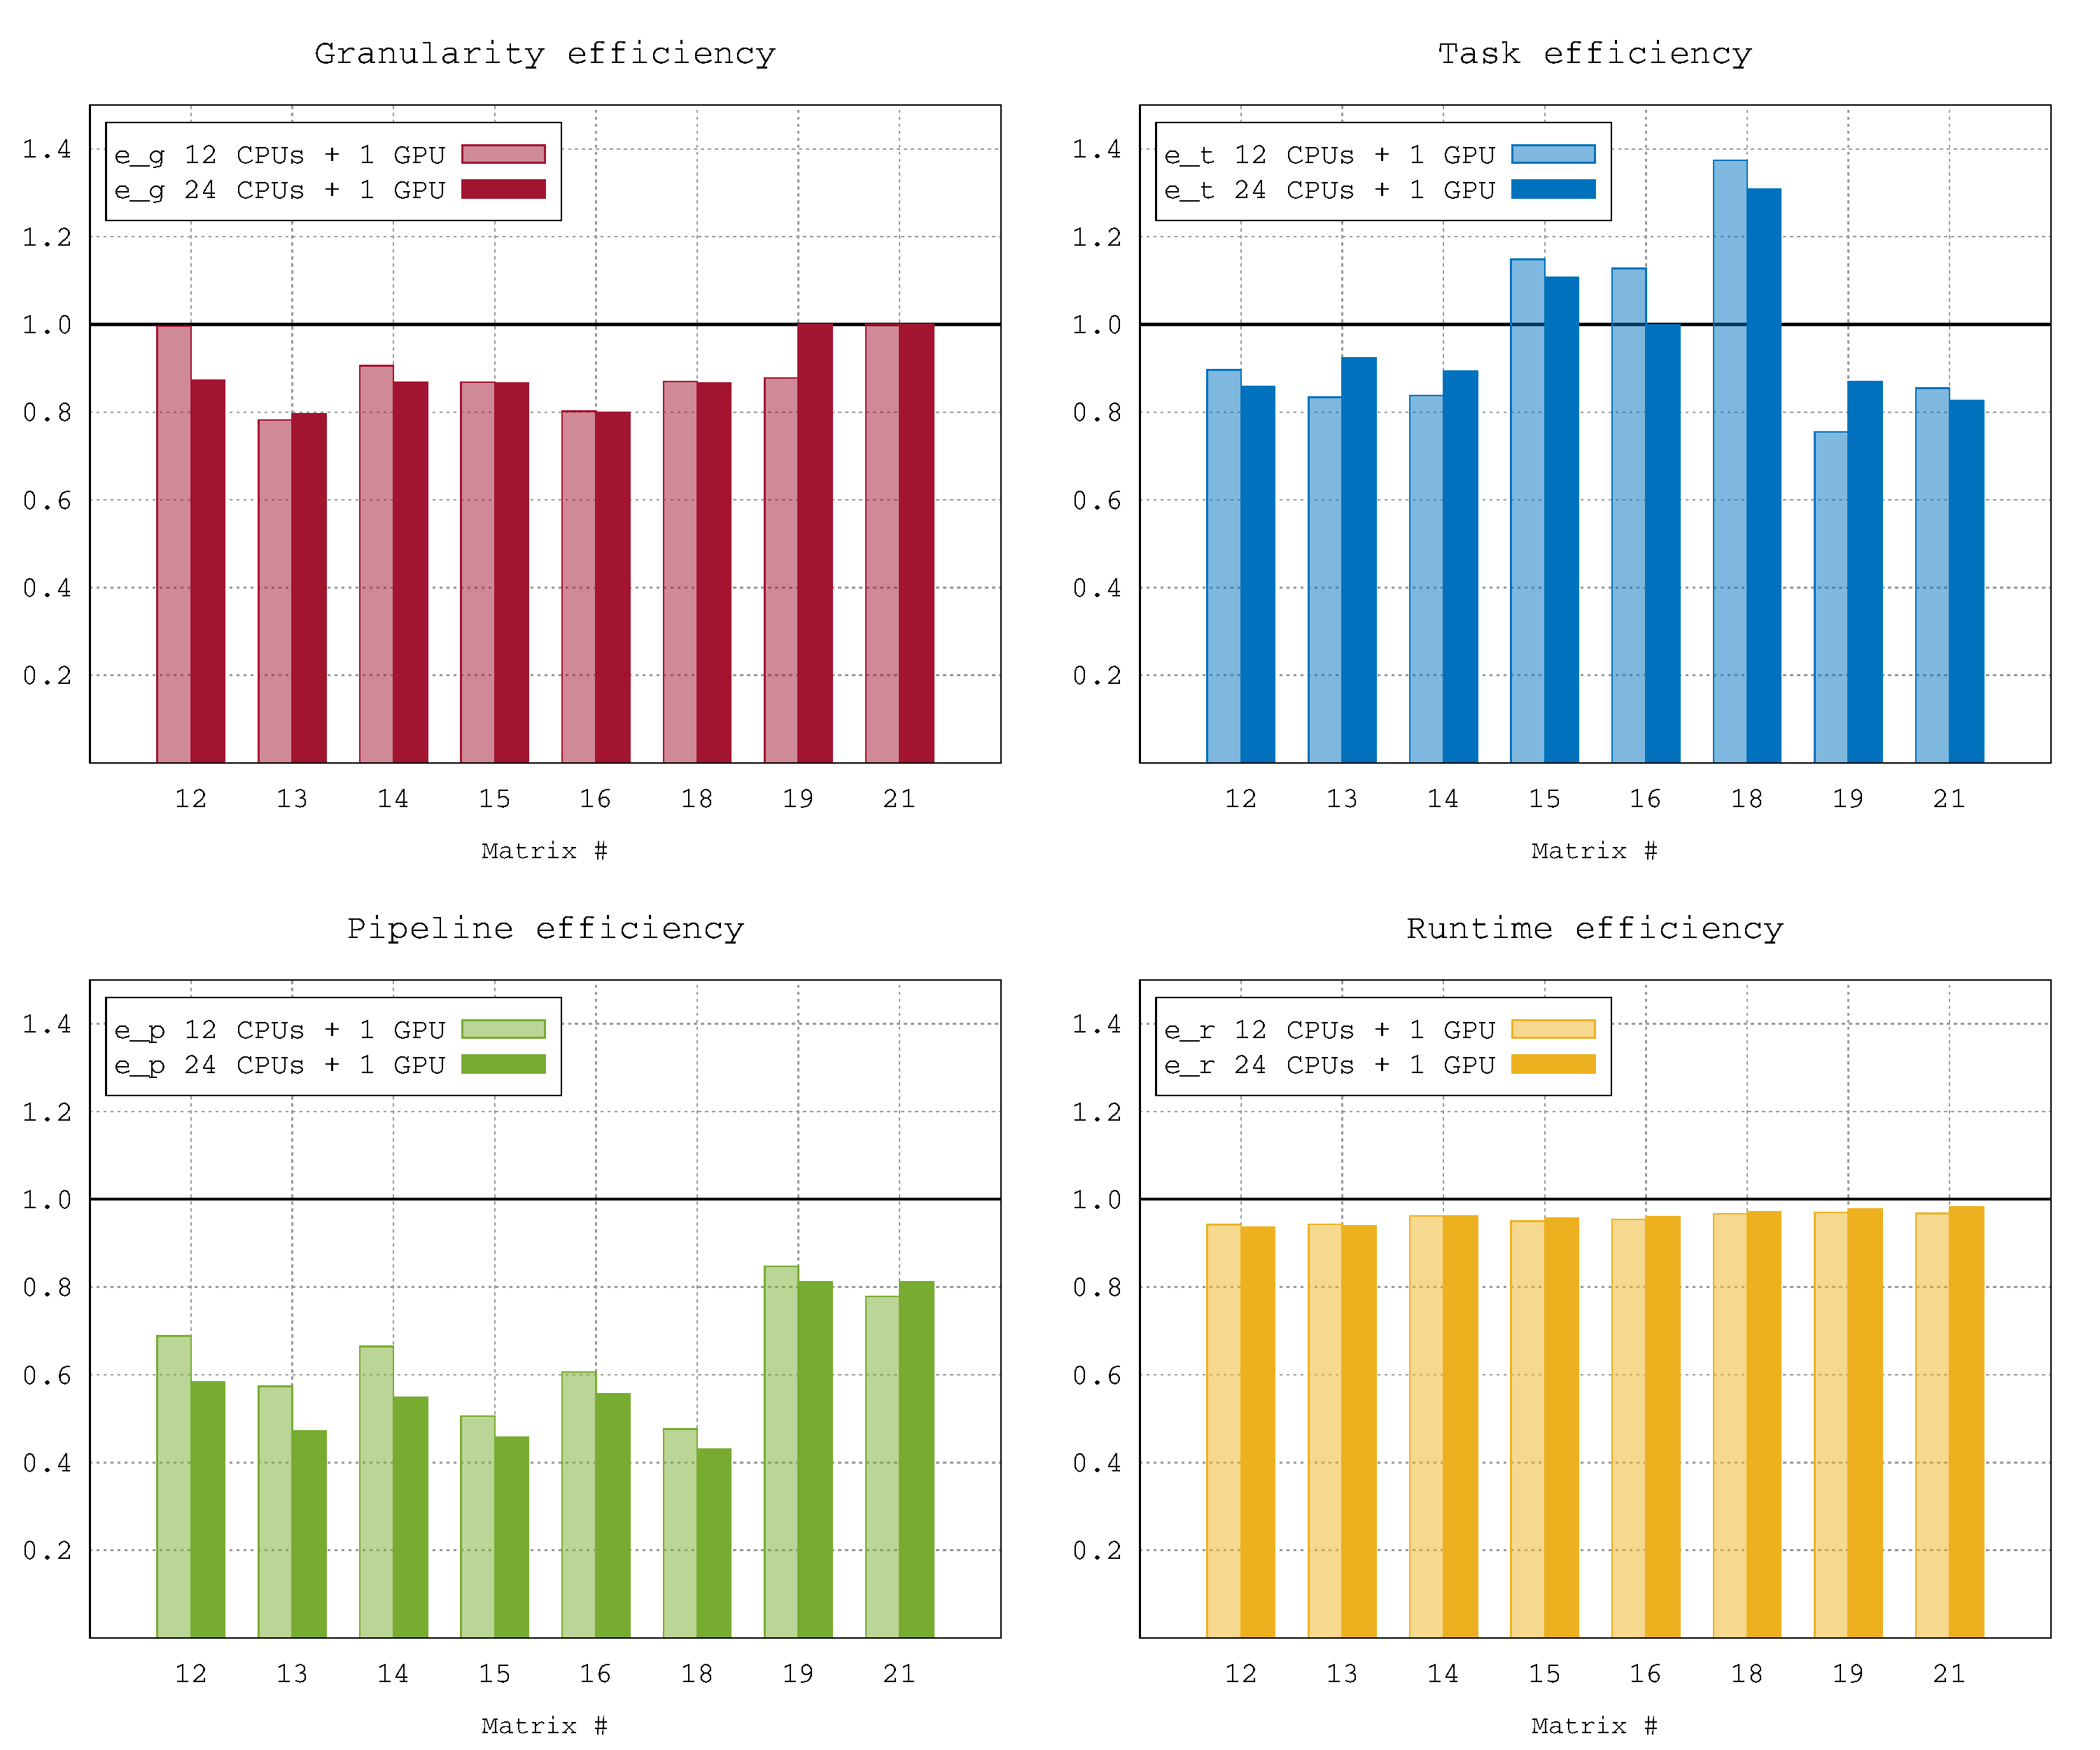
\includegraphics[width=0.9\textwidth]{data/eff_sirocco2}
\end{frame}

\begin{frame}{Experimental results: efficiency breakdown}
  \centering
  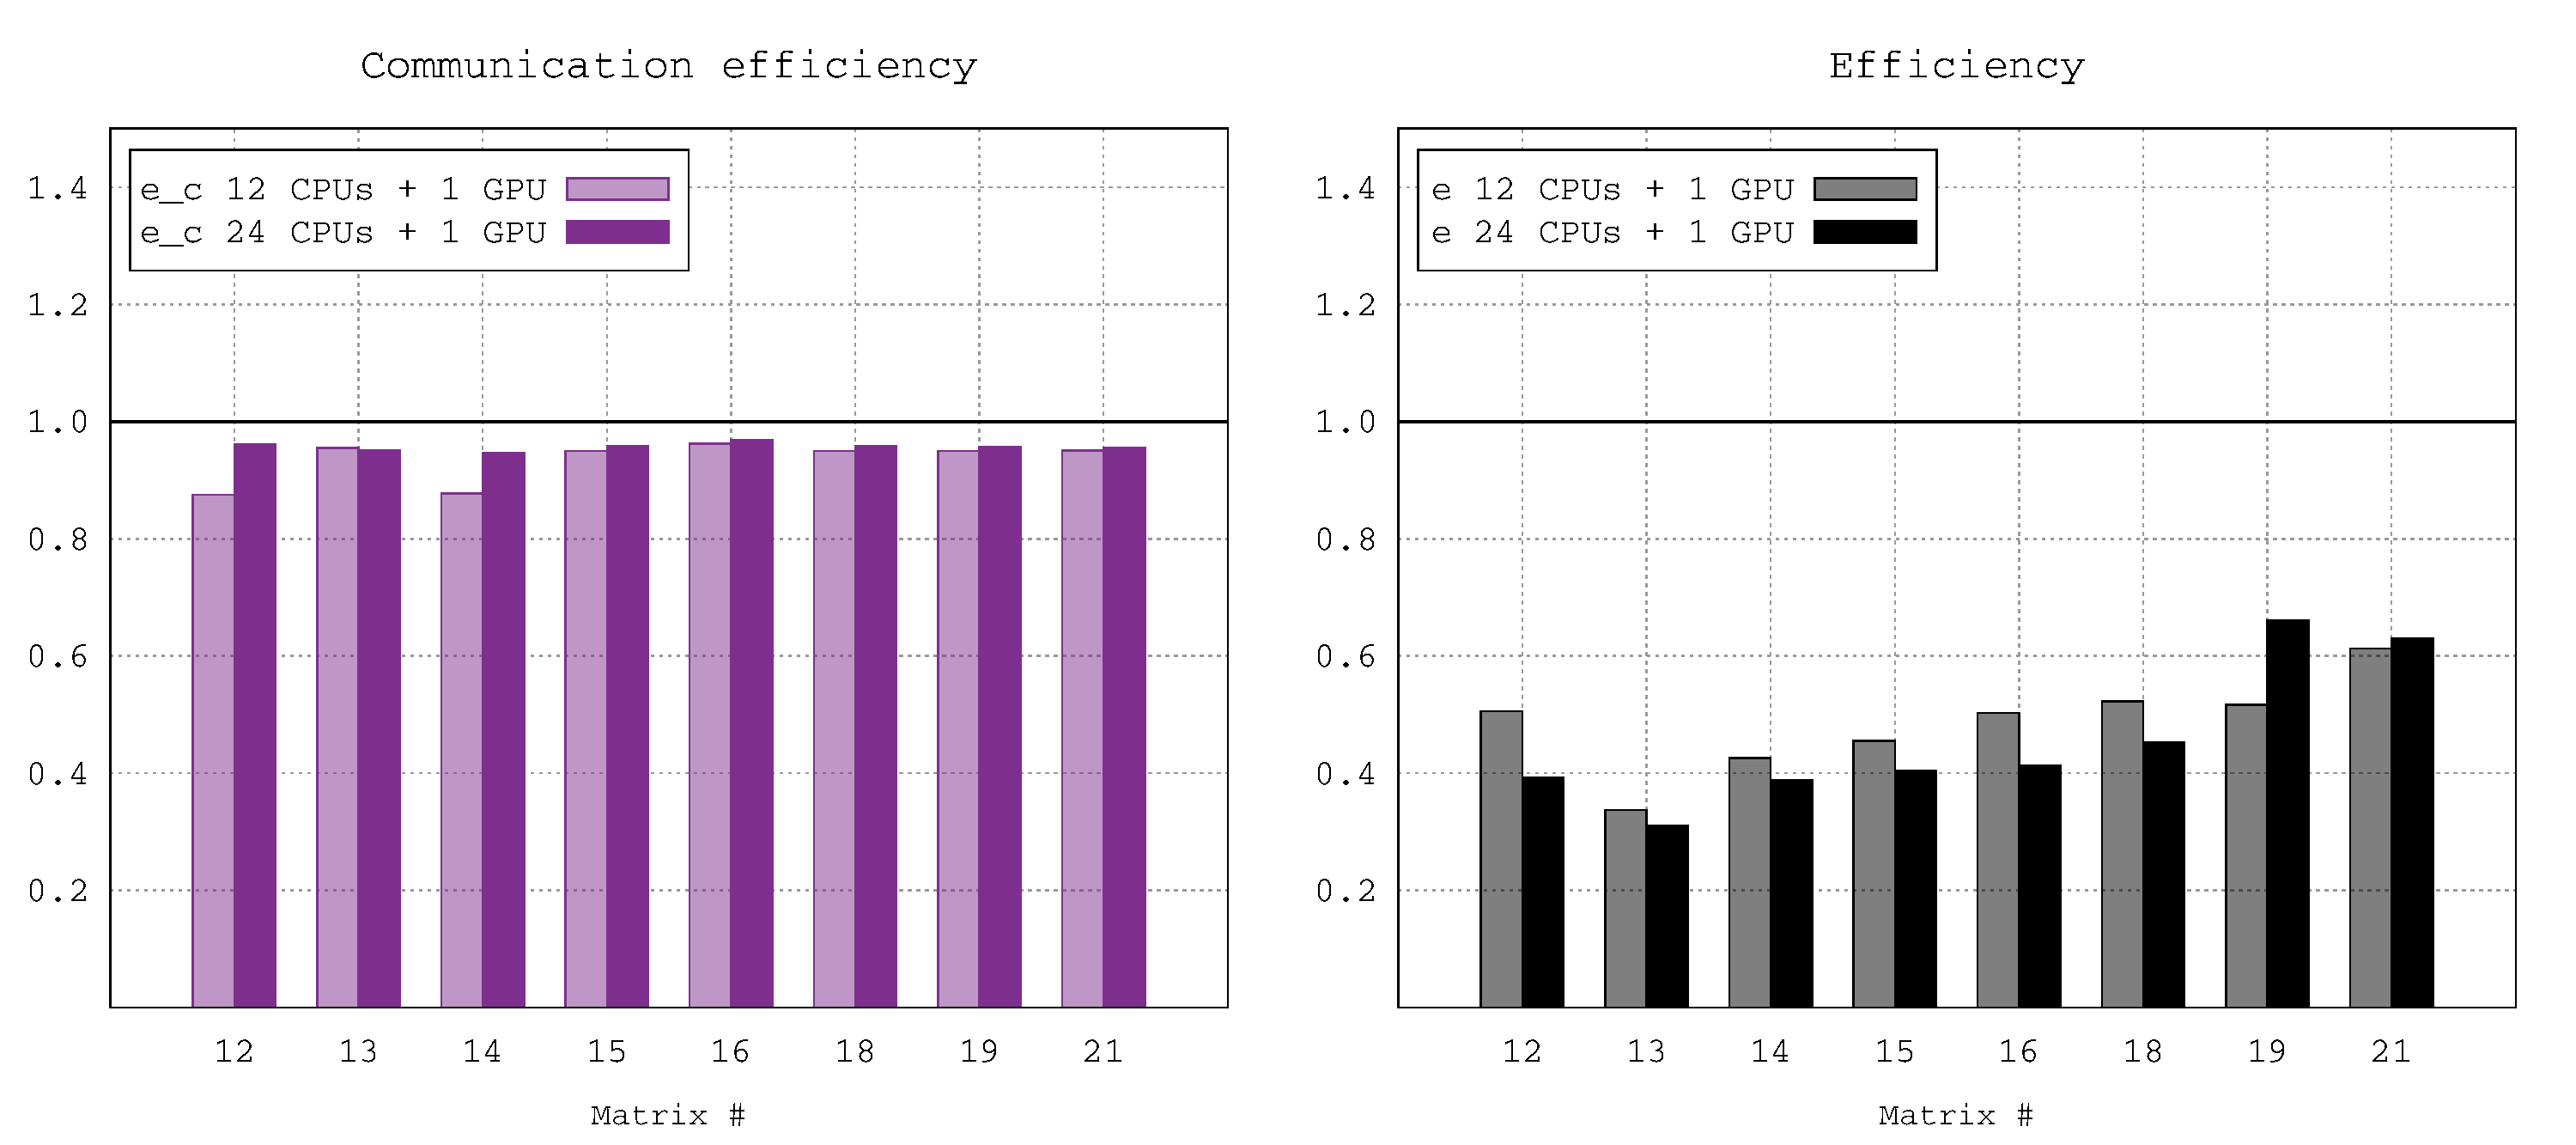
\includegraphics[width=0.9\textwidth]{data/eff_sirocco3}
\end{frame}

\begin{frame}{Experimental results: absolute performance}
  \centering
  \only<1>{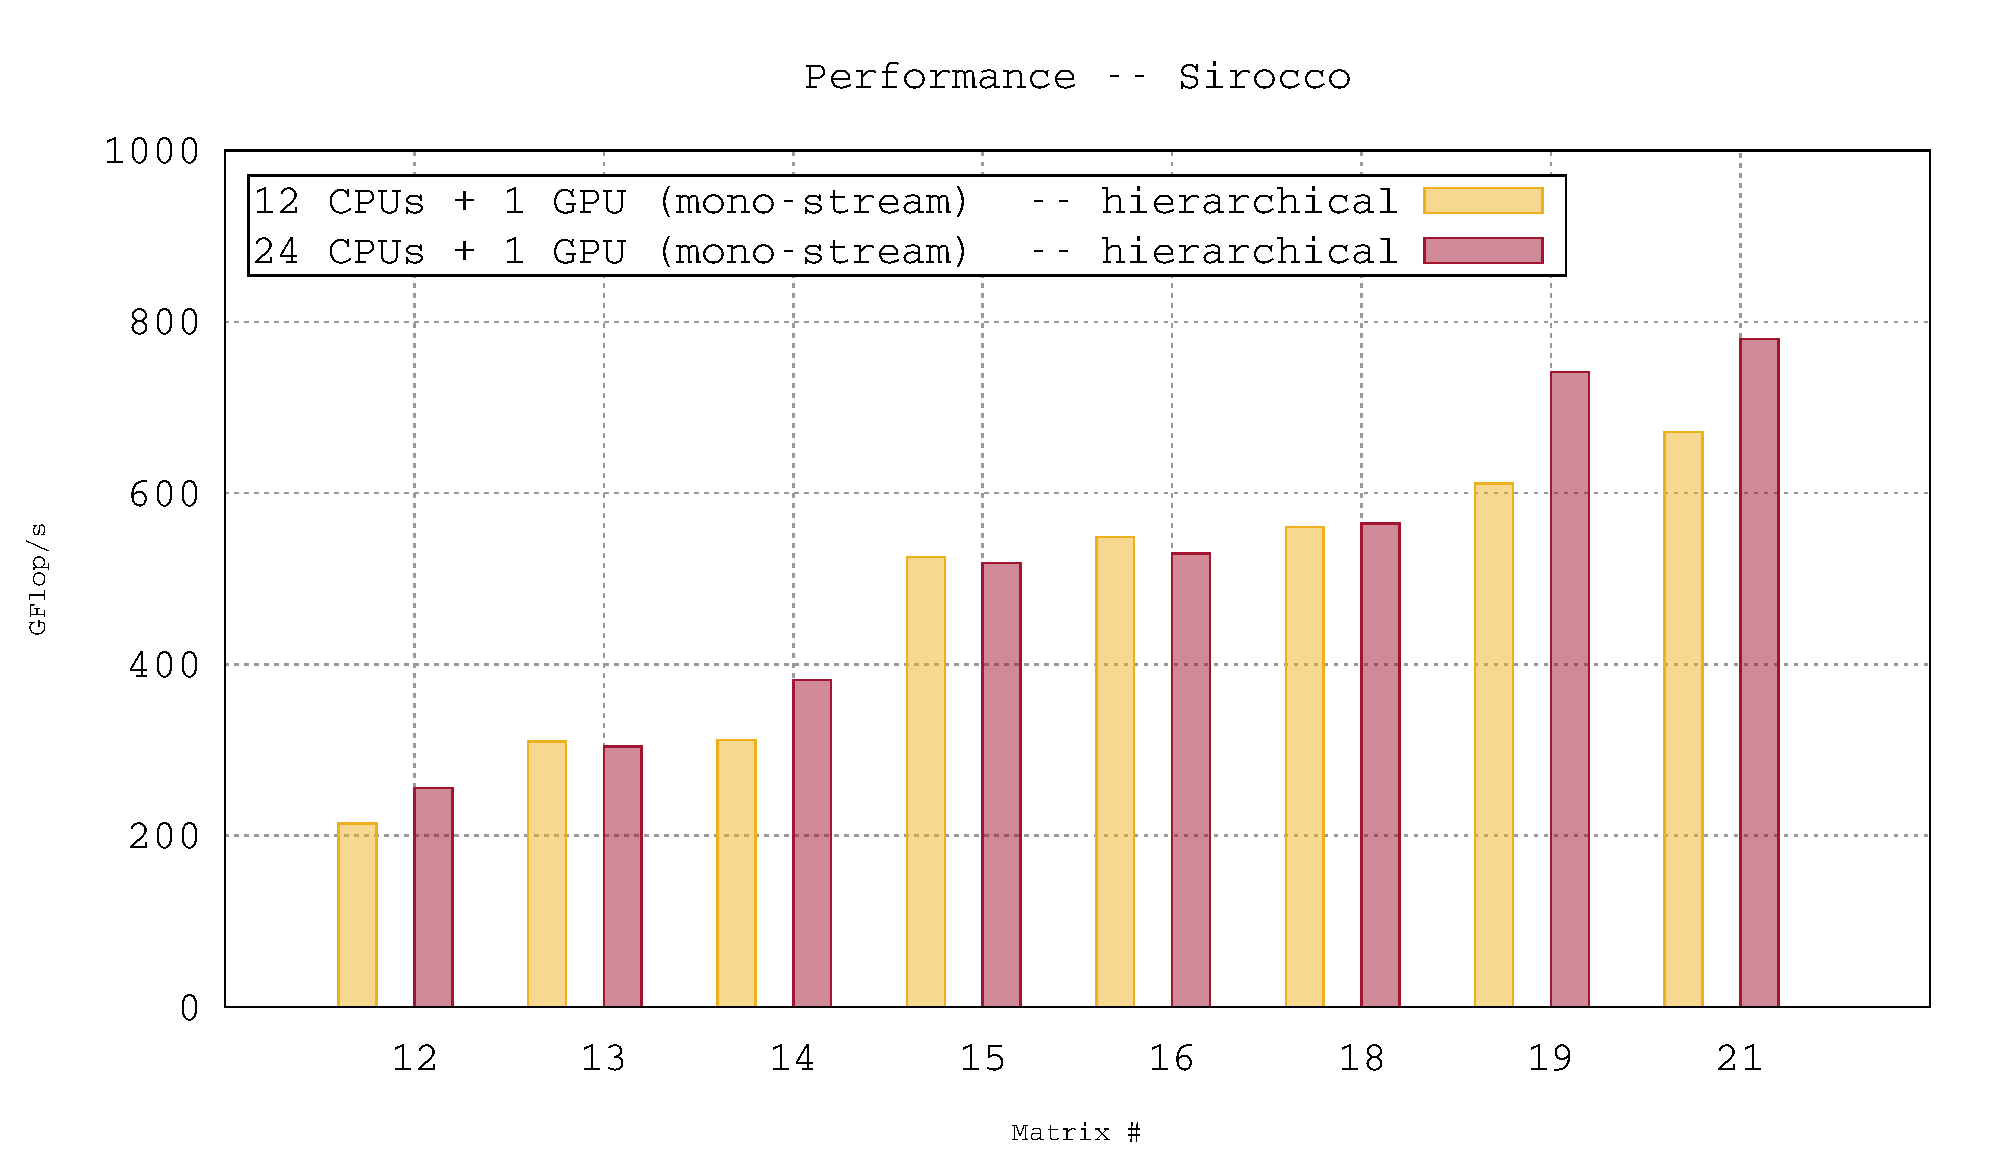
\includegraphics[width=0.9\textwidth]{data/perf_multistream_sirocco2_1}}
  \only<2>{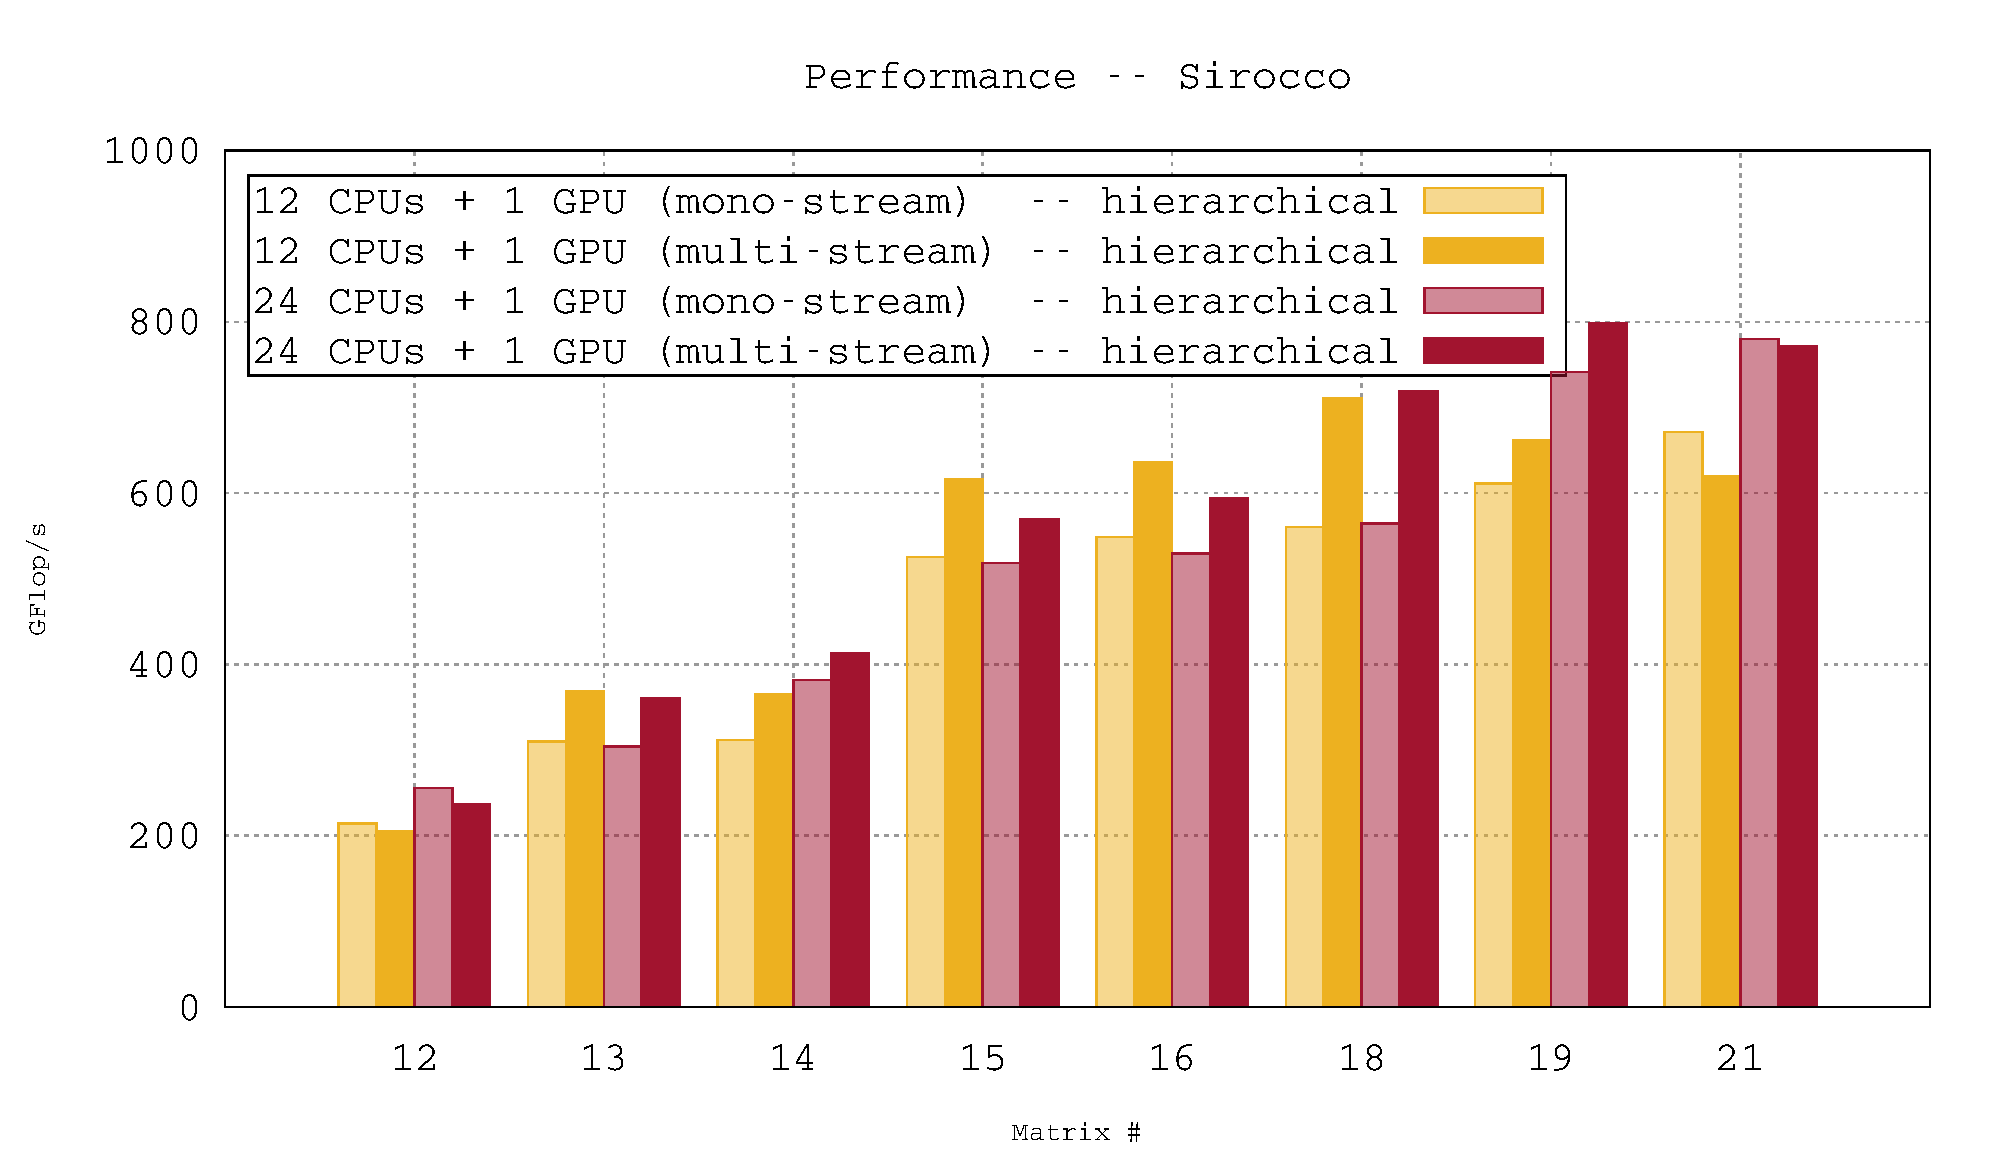
\includegraphics[width=0.9\textwidth]{data/perf_multistream_sirocco2_2}}

  \begin{itemize}
  \item A \dr{stream} is a sequence of commands that execute in order;
  \item The use of multiple stream increases the \dr{occupancy} of the
    device;
  \item Note that tasks that whose execution cannot be overlapped are
    serialized on the GPU.
  \end{itemize}
\end{frame}

\begin{frame}{Performance of multifrontal QR factorization}

  Comparison with \alert{GPU-only} SuiteSparse QR (factorization time):

  \vspace{0.3cm}

  
  \begin{center}

\begin{table}[h]
  \centering
  \begin{tabular}{llrrr}
    \toprule
    \rowcolor{bgray}
    \# & \multicolumn{2}{c}{Factorize time (s)} \\
    \rowcolor{bgray}
       & \qrm      & \spqr                      \\
    \otoprule                                                      
    2  & 1.661E+00 & 3.210E+00                  \\
    5  & 4.164E+00 & 5.469E+00                  \\
    % 6  & 9.084E+00 & $\ast$                     \\
    24 & 8.893E+00 & 1.493E+01                  \\
    7  & 8.585E+00 & 1.874E+01                  \\
    8  & 1.652E+01 & 2.254E+01                  \\
    % 9  & 2.834E+01 & $\ast$                     \\
    11 & 6.001E+01 & $\ast\ast$                 \\
    \bottomrule
  \end{tabular}
  % \caption{\label{tab:comparison-factorize-times}Factorization time
  %   for the test matrices with \qrm (24 CPU cores and 1 GPU) using
  %   multiple streams. On the last column, the factorization times for
  %   the \spqr solver. $\ast$ means that the solver returned an
  %   erroneous solution and $\ast\ast$ means that the memory
  %   requirement for these matrices  exceeded the GPU memory size.}
\end{table}

    % \begin{tabular}{l|rrrrr}
    %   \toprule
    %   & \multicolumn{5}{c}{Matrix \#}                                                                                                        \\
    %   \cmidrule(r){2-6}
    %   & 1                       & 2                       & 4                        & 5                         & 6                         \\
    %   \hline
    %   \qrm 1 stream & 2.4                     & 6.2                     & \cellcolor{gray!20}  9.4 & \cellcolor{gray!20}  14.4 & \cellcolor{gray!20}  19.8 \\
    %   \qrm 2 stream & \cellcolor{gray!20} 2.4 & 6.6                     & 10.7                     & 14.9                      & 20.6                      \\
    %   \spqr         & 2.7                     & \cellcolor{gray!20} 5.2 & 14.3                     & 18.2                      & 22.0                      \\
    %   \bottomrule
    % \end{tabular}
  \end{center}

  \begin{itemize}
  \item \qrm is competitive with a \alert{GPU-only} code despite the
    data movements.
  \item performance difference due to the use of CPUs.
  % \item on matrices 3 and 7 \spqr returned an incorrect result (likely
  %   due to a misuse of the software?).
  \item on matrices \# 11 \spqr run out of GPU memory:
    \begin{itemize}
    \item SPQR limited by maximum front (family) size.
    \item \qrm limited by maximum task size.
    % \item GPU memory is managed by the runtime system.
    \end{itemize}
  \end{itemize}

\end{frame}

%%% Local Variables:
%%% mode: latex
%%% TeX-master: "defense"
%%% TeX-engine: xetex
%%% End:
